% this package is designed by: thanhhungqb@gmail.com
% more infor mation and update: 
%   https://github.com/thanhhungqb/thesis-template

\documentclass[12pt,a4paper,oneside]{book} % twoside for draf

%\usepackage{babel}
\usepackage[utf8]{vietnam}
%\usepackage{times}
%\usepackage{graphicx}

\usepackage{mathptmx}	% same Time New Roma
%\renewcommand{\rmdefault}{phv} % Arial
%\renewcommand{\sfdefault}{phv} % Arial

\usepackage{fancyhdr}
\usepackage{algorithm2e}

\usepackage{thesis}

%\csdeptname{KHOA ĐIỆN ĐIỆN TỬ}
%\crname{BÁO CÁO THỰC TẬP TỐT NGHIỆP}
% \crname{BÁO CÁO TIỂU LUẬN}
\title{TIỀN XỬ LÝ DỮ LIỆU VỚI PYTHON}
\csCouncil{Khoa học máy tính}
\csSupervise{ThS. Nguyễn Mạnh Hùng}
\csReviewer{ThS. Nguyễn Mạnh Hùng}
\cttime{11/2022}

\thesislayout

\begin{document}
%-	Bìa cứng - màu xanh dương, chữ mạ vàng (xem mẫu đính kèm)
%-	Trang tên (tờ lót): chất liệu giấy, nội dung giống như bìa LV
%-	Ở gáy LV: in nhan đề LV (có thể in tóm tắt nếu nhan đề quá dài), size 15 – 17
%-	Phiếu Nhiệm vụ LV, chấm điểm Hướng dẫn & Phản biện (đã ký): nhận từ GVHD & GVPB sau khi bảo vệ (theo lịch hẹn).
%-	Lời cam đoan
%-	Lời cảm ơn/ Lời ngỏ
%-	Tóm tắt LV
%-	Mục lục
%-	Danh mục, bảng biểu, hình ảnh, ... (nếu có)
%-	Nội dung LV
%-	Danh mục TL tham khảo
%-	Phụ lục (nếu có)

\coverpage

\frontmatter



%-	Tóm tắt LV
\begin{abstract}
	Phần nhiều khối lượng công việc của phân tích và mô hình hóa dữ liệu nằm ở việc chuẩn bị, hay còn gọi là tiền xử lý dữ liệu: vận hành, sàng lọc, biến đổi và sắp xếp dữ liệu. Cách thức mà dữ liệu được lưu trữ và sắp xếp trong tập tin hoặc database không phải lúc nào cũng thuận tiện hoàn hảo cho ứng dụng xử lý dữ liệu.  Cách xử lý dữ liệu theo kiểu chuyển đổi định dạng được sử dụng rộng rãi bởi mọi người với các ngôn ngữ đa dụng như Python, Perl, R hoặc Java. May mắn thay Python có một thư viện chuẩn tên Pandas cung cấp cho người dùng các công cụ hiệu quả và linh hoạt bậc cao, áp dụng cho nhiều thuật toán, hỗ trợ người dùng xử lý dữ liệu theo nhu cầu một cách dễ dàng. Phần báo cáo này sẽ cung cấp cho người đọc các phương pháp cơ bản với tiền xử lý dữ liệu sử dụng thư viện Pandas của Python.
\end{abstract}	
	
\tableofcontents
%\listofsymbols
\listoftables


%\listofalgorithms


\mainmatter

\fancyhead{}  % Clears all page headers and footers
%\rhead{\thepage}  % Sets the right side header to show the page number
%\lhead{}  % Clears the left side page header
%\fancyfoot[positions]{footer}
\renewcommand{\footrulewidth}{0.4pt}

\pagestyle{fancy}  % Finally, use the "fancy" page style to implement the FancyHdr headers

%Nội dung của chương sẽ ghi vào đây, sau đó import vào main
%Combining and Merging Data Sets : 2 người
%Người 1: Database-Style Dataframe Merges đến hết Concatenating Along an Axis
%Người 2: Combining Data Overlap đến Chapter3: hết Replacing Values
\chapter{KẾT HỢP VÀ GỘP CÁC TẬP DỮ LIỆU}
\begin{introchap1}
    Dữ liệu lưu trữ trong các đối tượng pandas có thể được gộp lại với nhiều cách đã được tích hợp sẵn trong thư viện này:\par
    \hfill\begin{minipage}{\dimexpr\textwidth-1cm}
\xdef\tpd{\the\prevdepth}
    $\bullet$\textbf{pandas.merge}
   nối các hàng trong các DataFrames dựa trên một hoặc nhiều từ khóa. Cách kết nối này khá quen thuộc với người sử dụng SQL hoặc các cơ sở dữ liệu kiểu khác vì cách dùng toán tử join của cơ sở dữ liệu .\par
   $\bullet$\textbf{pandas.concat}
   nối hoặc xếp các đối tượng dọc theo một cột.\par
   $\bullet$\textbf{combinefirst} 
   phương thức cho cắt lát các dữ liệu chồng lặp để tìm ra giá trị cho các ô trống trong một đối tượng với giá trị của các đối tượng khác.\par
\end{minipage}
    Phần báo cáo này sẽ đề cập đến tất cả các phương thức trên và đưa ra các ví dụ. Tất cả đều được tối ưu trong trong phần báo cáo này.
\end{introchap1}

\sffamily
%Người 1 bắt đầu làm ở đây
%Database-style DataFrame Merges, trang 178
\section{Gộp các tập dữ liệu DataFrame}
Các phương thức Merge hoặc Join kết hợp các tập dữ liệu bằng cách kết nối các hàng sử dụng một hoặc nhiều từ khóa.Các toán tử này là trung tâm của các tập dữ liệu tương quan. Hàm \textbf{merge} trong pandas là cách chính để sử dụng các thuật toán này trong dữ liệu của người dùng.\par
Hãy bắt đầu với một ví dụ đơn giản:\par
    \quad\textup{In [15]: df1 = DataFrame({'key': ['b','b','a','c','c','a','a','b'], 'data1': range(7)})}\par
    \par
    \quad\textup{In [16]: df2 = DataFrame({'key': ['b','a','d'], 'data2': range(3)})}\par
    Đây là một ví dụ của trường hợp gộp nhiều tập dữ liệu thành một; tập dữ liệu trong \textup{df1} có nhiều hàng được gán nhãn \textup{a} và \textup{b}, trong khi \textup{df2} có mỗi 1 hàng cho mỗi giá trị trong cột key của nó. Gọi \textbf{merge} với mỗi đối tượng trên ta nhận được \par
    \quad\textup{In [19]: pd.merge(df1, df2)}\par
    \quad\textup{Out [19]: }\par
    \quad\quad\textup{data1 key\quad data2}\par
    \quad0 \quad\quad 2 \quad a \quad\quad 0\par
    \quad1 \quad\quad 4 \quad a \quad\quad 0\par
    \quad2 \quad\quad 5 \quad a \quad\quad 0\par
    \quad3 \quad\quad 0 \quad b \quad\quad 1\par
    \quad4 \quad\quad 1 \quad b \quad\quad 1\par
    \quad5 \quad\quad 6 \quad b \quad\quad 1\par
Để ý rằng ta không xác định cụ thể cột nào để dồn chúng lại. Nếu không xác định cụ thể, \textbf{merge} sử dụng các cột có tên lặp chồng làm các từ khóa. Đây là một bài tập tốt để xác định sự khác biệt, ví dụ: \par
    \quad\textup{In [20]: pd.merge(df1, df2,on='key')}\par
    \quad\textup{Out [20]: }\par
    \quad\quad\textup{data1 key\quad data2}\par
    \quad0 \quad\quad 2 \quad a \quad\quad 0\par
    \quad1 \quad\quad 4 \quad a \quad\quad 0\par
    \quad2 \quad\quad 5 \quad a \quad\quad 0\par
    \quad3 \quad\quad 0 \quad b \quad\quad 1\par
    \quad4 \quad\quad 1 \quad b \quad\quad 1\par
    \quad5 \quad\quad 6 \quad b \quad\quad 1\par
Nếu tên các cột khác nhau ở mỗi đối tượng, ta có thể xác định chúng riêng biệt: \par
   \quad\textup{In [21]: df3 = DataFrame({'key': ['b','b','a','c','c','a','a','b'], 'data1': range(7)})}\par
   \quad\textup{In [22]: df4 = DataFrame({'rkey': ['a','b','d'], 'data2': range(3)})}\par
   \quad\textup{In [23]: pd.merge(df3, df4, leftOn='lkey', rightOn='rkey')}\par
    \quad\textup{Out [23]: }\par 
    \quad\quad\textup{data1 lkey\quad data2 \quad rkey}\par
    \quad0 \quad\quad 2 \quad a \quad\quad 0\quad\quad\quad a\par
    \quad1 \quad\quad 4 \quad a \quad\quad 0\quad\quad\quad a\par
    \quad2 \quad\quad 5 \quad a \quad\quad 0\quad\quad\quad a\par
    \quad3 \quad\quad 0 \quad b \quad\quad 1\quad\quad\quad b\par
    \quad4 \quad\quad 1 \quad b \quad\quad 1\quad\quad\quad b\par
    \quad5 \quad\quad 6 \quad b \quad\quad 1\quad\quad\quad b\par
Ta nhận ra 2 khóa 'c' và 'd' và các dữ liệu liên quan đều bị thiếu trong phần đầu ra. Bởi \textbf{merge} thực hiện dồn trong \textbf{'inner'}; từ khóa trong kết quả đầu ra là các phần giao thoa của 2 tập dữ liệu. Các lựa chọn có thể khác đó là \textbf{'left'}, \textbf{'right'}, và \textbf{'outer'}. Lựa chọn gộp \textbf{'outer'} hay nói cách khác là gộp kiểu ngoài, là kiểu gộp lấy phần gộp của các từ khóa, kết hợp gộp cả 2 tập dữ liệu lại:\par
    \quad\textup{In [24]: pd.merge(df1 df2, how='outer')}\par
    \quad\textup{Out[24]:}\par
    \quad\quad\textup{data1 key\quad data2}\par
    \quad0 \quad\quad 2 \quad a \quad\quad 0\par
    \quad1 \quad\quad 4 \quad a \quad\quad 0\par
    \quad2 \quad\quad 5 \quad a \quad\quad 0\par
    \quad3 \quad\quad 0 \quad b \quad\quad 1\par
    \quad4 \quad\quad 1 \quad b \quad\quad 1\par
    \quad5 \quad\quad 6 \quad b \quad\quad 1\par
    \quad6 \quad\quad 3 \quad b\quad NaN\par
    \quad7\quad NaN \quad c \quad\quad 2 \par
Để xác định kiểu kết hợp key nào sẽ hiển thị ở trong phần kết quả đầu ra phụ thuộc vào cách chọn trong phương thức merge, xét trường hợp nhiều từ khóa như việc hình thành một mảng các tuples để sử dụng như một từ khóa gộp riêng biệt(mặc dù cách thức gộp không hẳn là như vậy). \par
Vấn đề cuối cùng cần xem xét trong khi dùng các phương thức gộp đó là cách xử lý các cột có tên trùng lặp. Trong khi ta có thể chỉ đến vị trí trùng lặp một cách thủ công( trong phần đổi tên các cột ở sau này), \textbf{merge} có một lựa chọn cho chỉ cụ thể các chuỗi mang giá trị tên trùng lặp trong các DataFrame được gộp: \par
    \quad\textup{In [34]: pd.merge(df1 df2, how='outer')}\par
    \quad\textup{Out[34]:}\par
    \quad\quad\textup{ key1 key2x\quad lval\quad key2y \quad rval } \par
    \quad0 \quad bar \quad one \quad \quad 3 \quad one \quad \quad 6 \par
    \quad1 \quad bar \quad one \quad \quad 3 \quad two \quad \quad 7 \par
    \quad2 \quad foo \quad one \quad \quad 1 \quad one \quad \quad 4 \par
    \quad3 \quad foo \quad one \quad \quad 1 \quad one \quad \quad 5 \par
    \quad4 \quad foo \quad two \quad \quad 2 \quad one \quad \quad 4 \par
    \quad5 \quad foo \quad two \quad \quad 2 \quad one \quad \quad 5 \par

\quad\textup{In [35]: pd.merge(left, right, on='key1', suffixes=('Left','Right'))}\par
    \quad\textup{Out[35]:}\par
    \quad\quad\textup{ key1 key2Left\quad lval\quad key2Right\quad rval } \par
    \quad0 \quad bar \quad \quad one \quad \quad 3 \quad \quad \quad one \quad \quad 6 \par
   \quad1 \quad bar \quad \quad one \quad \quad 3 \quad \quad \quad two \quad \quad 7 \par
    \quad2 \quad foo \quad \quad one \quad \quad 1 \quad \quad \quad one \quad \quad 4 \par
   \quad3 \quad foo \quad \quad one \quad \quad 1 \quad \quad \quad one \quad \quad 5 \par
   \quad4 \quad foo \quad \quad two \quad \quad 2 \quad \quad \quad one \quad \quad 4 \par
   \quad5 \quad foo \quad \quad two \quad \quad 2 \quad \quad \quad one \quad \quad 5 \\ \par
Coi Bảng \textbf{1.1} để hiểu thêm về tham chiếu các đối số trong hàm \textbf{merge}. Gộp theo chỉ số sẽ là chủ để của phần tiếp theo  \par

\begin{table}[h]
\centering
    \begin{tabular}{l|p{10cm}}
      \textbf{ Tham số}  & \textbf{Mô tả} \\
left & DataFrame được gộp ở bên trái(đầu tiên) \\ 
right & DataFrame được gộp ở bên phải(sau )\\
how & Cách gộp, inner hay outer, left hay right, inner là mặc định  \\
on     &  Tên cột bắt đầu gộp, phải có ở cả 2 DataFrame.\\
left\_on   & Cột ở DataFrame bên trái để bắt đầu gộp \\
right\_on & Tương tự như left\_on đối với DataFrame bên phải  \\
left\_index   &  Chỉ số của cột DataFrame bên trái để bắt đầu gộp \\
right\_index & Tương tự như left\_index \\
sort  & Sắp xếp và lọc dữ liệu dựa theo các key \\
suffixes  & Các tupple chứa dữ liệu để thêm vào tên các cột bị chồng lặp \\
copy & Nếu giá trị này False thì tránh copy dữ liệu vào trong cấu trúc kết quả 
    \end{tabular}
    \caption{Các tham số của hàm \textbf{merge}}
    \label{tab:table1}
\end{table}


%Merging on Index, trang 182
\section{Gộp theo chỉ số}
Trong một số trường hợp, từ khóa gộp hay các từ khóa trong DataFrames sẽ là các chỉ số của các cột. Trong trường hợp này, ta có thể dùng \textbf{leftIndex=True} hoặc \textbf{rightIndex=True} hoặc cả hai để chỉ ra rằng chỉ số của các cột nên được dùng là các key: \par
    \quad\textup{In [36]: left1 = DataFrame({'key': ['a','b','a','a','a','b','c'],'value': range(6)})}\par

     \quad\textup{In [37]: right1 = $DataFrame({'group_val': [3.5, 7]}, index=['a', 'b'])$
}\par
     \quad\textup{In [38]: left1 }\par
     \quad\textup{In [39]: right1}\par
     \quad\textup{.....:}\par
     \quad\textup{Out[38]: \quad\quad\quad\quad\quad Out[39]:}\par
     \quad \quad key \quad value \quad \quad\quad\quad\quad groupVal \par
     \quad 0 \quad a \quad \quad \quad 0 \quad\quad\quad a \quad\quad\quad 3.5 \par
     \quad 1 \quad b \quad \quad \quad 1 \quad\quad\quad a \quad\quad\quad 7.0 \par
     \quad 2 \quad a \quad \quad \quad 2  \par
     \quad 3 \quad a \quad \quad \quad 3 \par
     \quad 4 \quad b \quad \quad \quad 4 \par
     \quad 5 \quad c \quad \quad \quad 5 \\ \par
     \quad\textup{In [40]: pd.merge(left1, right1, leftOn='key', rightIndex=True) }\par
    \quad\textup{Out[40]:}\par
    \quad \quad key \quad value \quad  groupVal \par
     \quad 0 \quad a \quad \quad \quad 0  \quad\quad\quad 3.5 \par
     \quad 1 \quad b \quad \quad \quad 1 \quad\quad\quad 3.5 \par
     \quad 2 \quad a \quad \quad \quad 2  \quad\quad\quad 3.5 \par
     \quad 3 \quad a \quad \quad \quad 3 \quad\quad\quad 7.0 \par
     \quad 4 \quad b \quad \quad \quad 4 \quad\quad\quad 7.0 \par
     \quad 5 \quad c \quad \quad \quad 5 \quad\quad\quad NaN \par
     Kỹ thuật đánh dấu dữ liệu theo cấp độ sẽ phức tạp hơn: \par
     \quad\textup{In [42]: lefth = DataFrame({'key1': ['Ohio', 'Ohio', 'Ohio', 'Nevada', 'Nevada'], }}\par
     \quad\quad\textup{.....: \quad\quad\quad\quad\quad\quad\quad\quad 'key2': [2000, 2001, 2002, 2001, 2002],}\par
     \quad\quad\textup{.....: \quad\quad\quad\quad\quad\quad\quad\quad 'data': np.arange(5.)}\par
    \quad\textup{In [44]: lefth}\par
    \quad\textup{n [45]: righth}\par
    \quad\textup{Out[44]: \quad\quad\quad\quad\quad Out[45]:}\par
     \quad \quad \quad data \quad\quad key1 \quad\quad key2 \quad\quad\quad\quad\quad\quad\quad\quad\quad\quad event1 \quad event2 \par
     \quad 0 \quad \quad \quad 0 \quad Ohio \quad\quad 2000 \quad \quad \quad Nevada 2001 \quad \quad \quad 0 \quad \quad \quad 1 \par
     \quad 1 \quad \quad \quad 1 \quad Ohio \quad\quad 2000 \quad \quad \quad Nevada 2000 \quad \quad \quad 0 \quad \quad \quad 3 \par
     \quad 2 \quad \quad \quad 2 \quad Ohio \quad\quad 2000 \quad \quad \quad Ohio\quad 2000 \quad \quad \quad 0 \quad \quad \quad 5 \par
     \quad 3 \quad \quad \quad 3 \quad Ohio \quad\quad 2000 \quad \quad \quad Ohio\quad 2000 \quad \quad \quad 0 \quad \quad \quad 7 \par
     \quad 4 \quad \quad \quad 4 \quad Ohio \quad\quad 2000 \quad \quad \quad Ohio\quad 2001 \quad \quad \quad 0 \quad \quad \quad 9 \par
     \quad  \quad \quad \quad  \quad \quad\quad \quad\quad\quad\quad \quad\quad \quad \quad \quad Ohio\quad 2002 \quad \quad \quad 10 \quad \quad  11 \\\par
     
     Trong trường hợp này, ta cần xác định nhiều cột để gộp thành một list(chú ý đến cách xử lý các chỉ số lặp): \par
     \quad\textup{In [46]: $pd.merge(lefth, righth, left_on=['key1', 'key2'], right_index=True)$}\par
     \quad\textup{Out[46]:}\par
     \quad \quad \quad data \quad\quad\quad key1 \quad\quad key2 \quad event1 \quad event2 \par
     \quad 3 \quad \quad \quad 3 \quad Nevada \quad\quad 2001 \quad \quad \quad 0 \quad \quad \quad 1 \par
     \quad 0 \quad \quad \quad 0 \quad\quad Ohio \quad\quad 2000 \quad \quad \quad 4 \quad \quad \quad 5 \par
     \quad 0 \quad \quad \quad 0 \quad\quad Ohio \quad\quad 2000 \quad \quad \quad 6 \quad \quad \quad 7 \par
     \quad 1 \quad \quad \quad 1 \quad\quad Ohio \quad\quad 2000 \quad \quad \quad 8 \quad \quad \quad 9 \par
     \quad 2 \quad \quad \quad 2 \quad\quad Ohio \quad\quad 2000 \quad \quad \quad 10 \quad \quad  11\\\par
     
     \quad\textup{In [47]: $pd.merge(lefth, righth, left_on=['key1', 'key2'],right_index=True, how='outer')$\\ \\ \\
}\par
     \quad\textup{Out[47]:}\par
    \quad \quad \quad data \quad\quad\quad key1 \quad\quad key2 \quad event1 \quad event2 \par
     \quad 4 \quad \quad NaN \quad Nevada \quad\quad 2000 \quad \quad \quad 2 \quad \quad \quad 3 \par
     \quad 3 \quad \quad \quad 3 \quad Nevada \quad\quad 2001 \quad \quad \quad 0 \quad \quad \quad 1 \par
     \quad 4 \quad \quad \quad 4 \quad\ Nevada  \quad\quad 2002 \quad \quad NaN \quad \quad NaN \par
     \quad 0 \quad \quad \quad 0 \quad\quad Ohio \quad\quad 2000 \quad \quad \quad 4 \quad \quad \quad 5 \par
     \quad 0 \quad \quad \quad 0 \quad\quad Ohio \quad\quad 2000 \quad \quad \quad 6 \quad \quad \quad 7 \par
     \quad 1 \quad \quad \quad 1 \quad\quad Ohio \quad\quad 2001 \quad \quad \quad 8 \quad \quad \quad 9 \par
     \quad 2 \quad \quad \quad 2 \quad\quad Ohio \quad\quad 2002 \quad \quad \quad 10 \quad \quad  11\\\par
     
     Sử dụng chỉ số của cả hai mảng hợp cũng không phải là một vấn đề quá khó: \par
     \quad\textup{In [48]: left2 = DataFrame([[1., 2.], [3., 4.], [5., 6.]], index=['a', 'c', 'e'],columns=['Ohio', 'Nevada'])}\par
     \quad\textup{In [49]: right2 = DataFrame([[7., 8.], [9., 10.], [11., 12.], [13, 14]],index=['b', 'c', 'd', 'e'], columns=['Missouri', 'Alabama'])}\par
     \quad\textup{In [50]: left2 \quad\quad\quad\quad\quad In [51]: right2}\par
     \quad\textup{Out[50]: \quad\quad \quad\quad\quad\quad\quad Out[51]:}\par
     \quad \quad  Ohio \quad Nevada \quad\quad\quad\quad \quad\quad Missouri \quad Alabama  \par
     \quad a \quad \quad 1 \quad\quad \quad 2 \quad\quad\quad\quad b \quad \quad \quad\quad 7 \quad \quad \quad\quad 8 \par
     \quad c \quad \quad 3 \quad\quad \quad 4 \quad\quad\quad\quad c \quad \quad \quad\quad 9 \quad \quad \quad\quad 10 \par
     \quad e \quad \quad 5 \quad\quad \quad 6 \quad\quad\quad\quad d \quad \quad \quad\quad 11 \quad \quad \quad\quad 12 \\ \par
    DataFrame có nhiều biến thể của \textbf{join} bằng cách gộp theo chỉ số. Ta cũng có thể gộp nhiều DataFrame bằng cách có nhiều chỉ số tương tự nhưng không chồng lặp các cột. Ở ví dụ trước, ta cũng có thể viết theo cách sau: \\ \par{}
    \quad\textup{In [53]: left2.join(right2, how='outer')}\par
    \quad\textup{Out[53]:}\par
    \quad \quad  Ohio \quad Nevada \quad\quad\quad\quad \quad\quad Missouri \quad Alabama  \par
     \quad a \quad \quad 1 \quad\quad \quad 2 \quad\quad\quad\quad b \quad \quad \quad\quad 7 \quad \quad \quad\quad 8 \par
     \quad c \quad \quad 3 \quad\quad \quad 4 \quad\quad\quad\quad c \quad \quad \quad\quad 9 \quad \quad \quad\quad 10 \par
     \quad e \quad \quad 5 \quad\quad \quad 6 \quad\quad\quad\quad d \quad \quad \quad\quad 11 \quad \quad \quad\quad 12 \\ \par
     Trong phần nguyên nhân thuộc tính, phương pháp \textbf{join} của DataFrame thực hiện gộp DataFrame đầu tiên theo các từ khóa. Phương thức này cũng hỗ trợ gộp theo chỉ số của DataFrame đã được tham chiếu đến dựa trên các cột của DataFrame được gọi: \par
     \quad\textup{In [54]: left1.join(right1, on='key')}\par
     \quad\textup{Out[54]:}\par
     \quad \quad key \quad value \quad  groupVal \par
     \quad 0 \quad a \quad \quad \quad 0  \quad\quad\quad 3.5 \par
     \quad 2 \quad a \quad \quad \quad 2 \quad\quad\quad 3.5 \par
     \quad 3 \quad a \quad \quad \quad 3  \quad\quad\quad 3.5 \par
     \quad 1 \quad b \quad \quad \quad 1 \quad\quad\quad 7.0 \par
     \quad 4 \quad b \quad \quad \quad 4 \quad\quad\quad 7.0 \par
     \quad 5 \quad c \quad \quad \quad 5 \quad\quad\quad NaN \\\par
    Cuối cùng, để gộp chỉ số theo chỉ số ta cần truyền vào một list các DataFrame để gộp theo cách tương tự dùng phương thức gộp chung được mô tả dưới đây: \par
    \quad\textup{In [55]: another = DataFrame([[7., 8.], [9., 10.], [11., 12.], [16., 17.]],
}\par
    \quad\textup{\quad\quad....: \quad\quad\quad\quad\quad index=['a', 'c', 'e', 'f'], columns=['New York', 'Oregon']),
}\\\par
    \quad\textup{In [56]: left2.join([right2, another])}\par
    \quad\textup{Out[56]:
}\par
    \quad\textup{Out[56]:}\par
    \quad \quad  Ohio \quad Nevada\quad Missouri \quad Alabama \quad New York \quad Oregon  \par
     \quad a \quad \quad 1 \quad\quad \quad 2 \quad\quad\quad NaN \quad \quad \quad NaN \quad \quad \quad\quad 7 \quad\quad\quad8  \par
     \quad c \quad \quad 3 \quad\quad \quad 4 \quad\quad\quad\quad 9 \quad \quad \quad \quad 10 \quad \quad \quad\quad 9 \quad\quad\quad 10  \par
      \quad e \quad \quad 5 \quad\quad \quad 6 \quad\quad\quad\quad 13 \quad \quad \quad  14 \quad \quad \quad\quad 11 \quad\quad\quad 12  \par
%Xong phần 1

%Người 2 bắt đầu làm ở đây
%Concatenating Along on Axis, trang 185
\section{Nối các tập dữ liệu theo cột}
    Một cách khác để kết hợp dữ liệu là ghép nối, liên kết hoặc xếp chồng. NumPy có chức năng nối để thực hiện việc này với các mảng NumPy thô: \par
    \quad\textup In [58]: arr = np.arange(12).reshape((3, 4))\par
    \quad\textup In [59]: arr \par
    \quad\textup Out[59]: \par
    \quad\textup array([[0, 1, 2, 3],\par
    \quad\quad\quad\quad\textup[4, 5, 6, 7],\par
    \quad\quad\quad\quad\textup[8, 9, 10, 11]])\par
    \quad\textup In [60]: np.concatenate([arr, arr], axis=1)\par
    \quad\textup Out[60]:\par
    \quad\textup array([[ 0, 1, 2, 3, 0, 1, 2, 3],\par
    \quad\quad\quad\quad\textup[4, 5, 6, 7, 4, 5, 6, 7],\par
    \quad\quad\quad\quad\textup[8, 9, 10, 11, 8, 9, 10, 11]])\par
    Trong ngữ cảnh của các đối tượng gấu trúc như Sê-ri và DataFrame, việc có các trục được gắn nhãn cho phép bạn khái quát hóa hơn nữa phép nối mảng. Đặc biệt, bạn có một số điều bổ sung để suy nghĩ về:\par
 $\bullet$ Nếu các đối tượng được lập chỉ mục khác nhau trên các trục khác, thì bộ sưu tập của các trục được hợp nhất hoặc giao nhau? \par
  $\bullet$ Các nhóm có cần được xác định trong đối tượng kết quả không \par
  $\bullet$  Trục nối có quan trọng không? \par
    Hàm concat trong pandas cung cấp một cách nhất quán để giải quyết từng mối quan tâm này. Tôi sẽ đưa ra một số ví dụ để minh họa cách nó hoạt động. Giả sử chúng ta có ba Sê-ri không có chỉ số trùng nhau: 
    \par\quad\textup In [61]: s1 = Series([0, 1], index=['a', 'b'])
    \par\quad\textup In [62]: s2 = Series([2, 3, 4], index=['c', 'd', 'e'])
    \par\quad\textup In [63]: s3 = Series([5, 6], index=['f', 'g'])
    \par Gọi concat với các đối tượng này trong danh sách sẽ dán các giá trị và chỉ mục lại với nhau: 
    \par\quad\textup In [64]: pd.concat([s1, s2, s3])
    \par\quad\textup Out[64]: 
    \par\quad\textup a 0
    \par\quad\textup b 1
    \par\quad\textup c 2
    \par\quad\textup d 3
    \par\quad\textup e 4
    \par\quad\textup f 5
    \par\quad\textup g 6
    \par Theo mặc định, concat hoạt động dọc theo trục = 0, tạo ra một series khác. Nếu bạn vượt qua axis=1, thay vào đó, kết quả sẽ là một DataFrame (trục = 1 là các cột):
    \par\quad\textup  In [65]: pd.concat([s1, s2, s3], axis=1)
    \par\quad\textup Out[65]:
\par\quad\textup\quad\quad 0\quad\quad\quad\quad 1\quad\quad\quad\quad 2
\par\quad\textup a\quad\quad0\quad\quad NaN\quad\quad NaN
\par\quad\textup b\quad\quad1\quad\quad NaN\quad\quad NaN
\par\quad\textup c\quad NaN \quad\quad\quad2\quad\quad NaN
\par\quad\textup d\quad NaN \quad\quad\quad3\quad\quad NaN
\par\quad\textup e\quad NaN \quad\quad\quad4\quad\quad NaN
\par\quad\textup f\quad NaN\quad\quad NaN\quad\quad\quad 5
\par\quad\textup g\quad NaN\quad\quad NaN\quad\quad\quad 6
    \par Trong trường hợp này, không có sự trùng lặp trên trục khác, như bạn có thể thấy là trục đã được sắp xếp union (nối 'bên ngoài' ) của các chỉ mục. Thay vào đó, bạn có thể cắt chúng bằng cách đi qua tham gia = 'bên trong':
    \par\quad\textup In [66]: s4 = pd.concat([s1 * 5, s3]) 
    \par\quad\textup In [67]: pd.concat([s1, s4], axis=1) \quad\quad\quad In [68]: pd.concat([s1, s4], axis=1, join='inner') 
    \par\quad\textup Out[67]: \quad\quad\quad\quad\quad\quad\quad\quad\quad\quad\quad\quad\quad \xspace Out[68]:
    \par\quad\quad\xspace\xspace 0\xspace 1 \quad\quad\quad\quad\quad\quad\quad\quad\quad\quad\quad\quad\quad\quad\xspace 0\xspace 1
    \par\quad\textup a\quad 0 0\quad\quad\quad\quad\quad\quad\quad\quad\quad\quad\quad\quad\quad\quad a 0 0
\par\quad\textup b\quad 1 5\quad\quad\quad\quad\quad\quad\quad\quad\quad\quad\quad\quad\quad\quad b 1 5
\par\quad\textup f NaN 5
\par\quad\textup g NaN 6
\par Bạn thậm chí có thể chỉ định các trục sẽ được sử dụng trên các trục khác với$ join_axe$s:
\par\quad\textup In [69]: $pd.concat([s1, s4], axis=1, join_axes=[['a', 'c', 'b', 'e']])$
\par\quad\textup Out[69]:
 \par\quad\quad\xspace\xspace 0\quad\xspace\xspace 1
\par\quad\textup a\quad 0\quad\xspace\xspace 0
\par\quad\textup c NaN NaN
\par\quad\textup b\quad 1\quad\xspace\xspace 5
\par\quad\textup e NaN NaN
    \par Một vấn đề là các phần được nối không thể xác định được trong kết quả. Giả sử thay vào đó, bạn muốn tạo một chỉ mục phân cấp trên trục nối. Để làm điều này,sử dụng đối số keys :
\par\quad\textup In [70]: result = pd.concat([s1, s1, s3], keys=['one', 'two', 'three'])
\par\quad\textup In [71]: result
\par\quad\textup Out[71]:
\par\quad\textup one\quad a\quad 0
\par\quad\textup\quad\quad\xspace b\quad 1
\par\quad\textup two\quad a\quad 0
\par\quad\textup\quad\quad\xspace b\quad 1
\par\quad\textup three f\quad 5
\par\quad\textup\quad\quad  g\quad 6
\par\quad\textup In [72]: $result.unstack()$
\par\par\par
\par\quad\textup Out[72]:


\par\quad\textup \quad\quad\quad\quad\quad\quad a \quad\quad\quad \quad b\quad\quad\quad  \quad\quad f\quad\quad\quad\quad\quad g
\par\quad\textup one \quad\quad\quad\quad 0\quad\quad\quad\quad  1\quad\quad\quad\quad  NaN\quad\quad\quad\quad  NaN
\par\quad\textup two \quad\quad\quad\quad 0 \quad\quad\quad\quad 1\quad\quad\quad\quad  NaN\quad\quad  NaN
\par\quad\textup  three \quad\quad\quad NaN \quad\quad NaN\quad\quad\quad\quad  5\quad\quad\quad\quad  6
\par Trong trường hợp kết hợp series dọc theo trục=1, các khóa trở thành tiêu đề cột DataFrame:
\par\quad\textup In [73]: pd.concat([s1, s2, s3], axis=1, keys=['one', 'two', 'three'])
\par\quad\textup Out[73]:
\par\quad\textup\quad   one\xspace two\xspace three
\par\quad\textup a\quad 0\quad NaN\xspace\xspace\xspace NaN
\par\quad\textup b\quad 1\quad NaN\xspace\xspace\xspace NaN
\par\quad\textup c NaN\quad\quad 2\xspace\xspace\xspace NaN
\par\quad\textup d NaN\quad\quad 3\xspace\xspace\xspace NaN
\par\quad\textup e NaN\quad\quad 4\xspace\xspace\xspace NaN
\par\quad\textup f NaN\quad NaN\quad\quad 5
\par\quad\textup g NaN\quad NaN\quad\quad 6
\par\quad\textup Logic tương tự mở rộng cho các đối tượng DataFrame:
\par\quad\textup In [74]: df1 = DataFrame(np.arange(6).reshape(3, 2), index=['a', 'b', 'c'],
\par\quad\textup  ....:\quad\quad\quad\quad  columns=['one', 'two'])
\par\quad\textup In [75]: df2 = DataFrame(5 + np.arange(4).reshape(2, 2), index=['a', 'c'],
\par\quad\textup ....: \quad\quad\quad\quad columns=['three', 'four'])
\par\quad\textup In [76]: pd.concat([df1, df2], axis=1, keys=['level1', 'level2'])
\par\quad\textup Out[76]:
\par\quad\textup\quad \quad\quad  level1 \quad\quad level2
\par\quad\textup \quad\quad\quad\quad  one \quad\quad\quad two\quad\quad\quad  three\quad\quad\quad four
\par\quad\textup a \quad\quad\quad\quad 0\quad\quad\quad\quad  1\quad\quad\quad\quad  5\quad\quad\quad\quad  6
\par\quad\textup b \quad\quad\quad\quad 2 \quad\quad\quad\quad 3\quad\quad\quad\quad  NaN\quad\quad  NaN
\par\quad\textup  c \quad\quad\quad\quad 4 \quad\quad\quad\quad 5\quad\quad\quad\quad  7\quad\quad\quad\quad  8
\par\quad\textup Nếu bạn chuyển một lệnh của các đối tượng thay vì một danh sách, các phím của lệnh đó sẽ được sử dụng cho tùy
chọn phím :
\par\quad\textup In [77]: pd.concat({'level1': df1, 'level2': df2}, axis=1)
\par\quad\textup Out[77]:
\par\quad\textup\quad\quad level1 level2
\par\quad\textup\quad\quad one\quad two\quad three \quad four
\par\quad\textup a\quad\quad 0\quad\quad 1\quad 5  \quad\quad\quad 6
\par\quad\textup b\quad\quad 2\quad\quad 3\quad NaN\quad\quad NaN
\par\quad\textup c\quad\quad 4\quad\quad 5\quad 7  \quad \quad\quad 8
\par\quad\textup Có một số đối số bổ sung chi phối cách tạo chỉ mục phân cấp (xem Bảng 7-2):
\par\quad\textup In [78]: pd.concat([df1, df2], axis=1, keys=['level1', 'level2'],
\par\quad\textup ....: \quad\quad names=['upper', 'lower'])
\par\quad\textup Out[78]:
\par\quad\textup upper level1 level2
\par\quad\textup lower one\quad two\quad three \quad four
\par\quad\textup a\quad\quad 0\quad\quad 1\quad 5  \quad\quad\quad 6
\par\quad\textup b\quad\quad 2\quad\quad 3\quad NaN\quad\quad NaN
\par\quad\textup c\quad\quad 4\quad\quad 5\quad 7  \quad \quad\quad 8
\par Cân nhắc cuối cùng liên quan đến DataFrames trong đó chỉ mục hàng không có ý nghĩa trong ngữ cảnh phân tích:
\par\quad\textup In [79]: df1 = DataFrame(np.random.randn(3, 4), columns=['a', 'b', 'c', 'd'])
\par\quad\textup In [80]: df2 = DataFrame(np.random.randn(2, 3), columns=['b', 'd', 'a'])
\par\quad\textup In [81]:\quad\quad\quad\quad df1 In [82]: df2
\par\quad\textup Out[81]:\quad\quad\quad\quad\quad\quad\quad\quad\quad\quad\quad\quad\quad\quad\quad\quad Out[82]:
\par\quad\textup \quad\quad\quad\quad a\quad\quad b\quad\quad\quad\quad c\quad\quad\quad\quad d \quad\quad\quad\quad\quad\quad b\quad\quad\quad\quad d\quad\quad\quad\quad a
\par\quad\textup 0 -0.204708 0.478943 -0.519439 -0.555730\quad\quad 0 0.274992 0.228913 1.352917
\par\quad\textup 1 1.965781 1.393406 0.092908  0.281746\quad\quad\quad 1 0.886429 -2.001637 -0.371843
\par\quad\textup 2 0.769023 1.246435 1.007189 -1.296221
\par\quad\textup Trong trường hợp này, bạn có thể bỏ qua $ignore_index=True$:
\par\quad\textup In [83]: $pd.concat([df1, df2], ignore_index=True)$
\par\quad\textup Out[83]:
\par\quad\quad\quad\quad\quad a \quad\quad\quad b\quad\quad\quad  c\quad\quad\quad  d
\par\quad 0 -0.204708 0.478943 -0.519439 -0.555730
\par\quad 1 1.965781 1.393406 0.092908 0.281746
\par\quad 2 0.769023 1.246435 1.007189 -1.296221
\par\quad 3 1.352917 0.274992\quad NaN\quad\quad 0.228913
\par\quad 4 -0.371843 0.886429\quad NaN\quad\quad -2.001637 \\ \par
\quad\textup{Bảng 7-2: tham số của hàm concat}
\begin{table}[h]
\centering
    \begin{tabular}{l|p{10cm}}
      \textbf{ Tham số}  & \textbf{Mô tả} \\
objs & Danh sách các dictionary của các đối tượng pandas để concat \\ 
axis & Cột để bắt đầu concat, mặc định là cột 0 \\
join  & Cách concat: inner hoặc outer, mặc định là outer  \\
join\_axes     &  Chỉ số cụ thể để dùng cho các cột n-1 khác ngoại trừ các hàm lấy phần chung.\\
keys   & Các giá trị để tham gia vào đối tượng được concat \\
levels & Các chỉ số cụ thể để sắp xếp theo thứ bậc   \\
names   &  Tên cho các bậc chỉ số nếu key được truyền vào \\
verify\_integrity  & Kiểm tra nếu cột trong đối tượng được concat có bị lặp \\
ignore\_index  & Không đảo ngược chỉ số theo các cột được concat, mà trả về range(total\_lenght)
\end{tabular}
    \caption{Các tham số của hàm \textbf{concat}}
    \label{tab:table2}
\end{table}
%Combining Data with Overlap, trang 188
\section{Kết hợp dữ liệu chéo}
\par\textup Tình huống kết hợp dữ liệu khác không thể được biểu thị dưới dạng thao tác hợp nhất hoặc nối quốc gia. Bạn có thể có hai tập dữ liệu có chỉ mục trùng nhau toàn bộ hoặc một phần. Như một ví dụ thúc đẩy, hãy xem xét hàm where của NumPy, biểu thị một if-else được vector hóa:
\par\quad\textup In [84]: a = Series([np.nan, 2.5, np.nan, 3.5, 4.5, np.nan],
\par\quad\quad\quad  ....:\quad\quad index=['f', 'e', 'd', 'c', 'b', 'a'])
\par\quad\textup In [85]: b = Series(np.arange(len(a), dtype=np.float64),
\par\quad\quad\quad ....:\quad\quad index=['f', 'e', 'd', 'c', 'b', 'a'])
\par\quad\textup In [86]: b[-1] = np.nan
\par\quad\textup In [87]: a\quad\quad\quad In [88]: b\quad\quad In [89]: np.where(pd.isnull(a), b, a)
\par\quad\textup Out[87]:\xspace\quad\quad\quad Out[88]:\quad\quad\quad Out[89]:
\par\quad\textup f NaN\xspace\xspace\xspace\quad\quad\quad\quad f 0\quad\quad\quad\quad\quad\xspace\quad f 0.0
\par\quad\textup e 2.5\quad\quad\quad\quad\quad e 1\quad\quad\quad\quad\quad\quad e 2.5
\par\quad\textup d NaN\xspace\xspace\quad\quad\quad\quad d 2\quad\quad\quad\quad\quad\quad d 2.0
\par\quad\textup c 3.5\quad\quad\quad\quad\quad c 3\quad\quad\quad\quad\quad\quad c 3.5
\par\quad\textup b 4.5\quad\quad\quad\quad\quad b 4\quad\quad\quad\quad\quad\quad b 4.5
\par\quad\textup a NaN\quad\quad\quad\quad a NaN\quad\quad\quad\quad\quad a NaN
\par\quad\textup Series có phương thức kết hợp đầu tiên , thực hiện tương đương với thao tác này cộng với căn chỉnh dữ liệu:
\par\quad\textup In [90]: $b[:-2].combine_first(a[2:])$
\par\quad\textup Out[90]:
\par\quad\textup a\quad NaN
\par\quad\textup b\quad 4.5
\par\quad\textup c\quad 3.0
\par\quad\textup d\quad 2.0
\par\quad\textup e\quad 1.0
\par\quad\textup f\quad 0.0
\par\quad\textup Với DataFrames, tổ hợp first tự nhiên thực hiện cùng một việc theo từng cột, vì vậy bạn
có thể coi đó là "vá" dữ liệu bị thiếu trong đối tượng gọi bằng dữ liệu từ đối tượng bạn
chuyển:
\par\quad\textup In [91]: df1 = DataFrame({'a': [1., np.nan, 5., np.nan],
\par\quad\textup\quad ....:\quad\quad\quad\quad\quad\quad\quad\quad 'b': [np.nan, 2., np.nan, 6.],
\par\quad\textup\quad  ....:\quad\quad\quad\quad\quad\quad\quad\quad 'c': range(2, 18, 4)})
\par\quad\textup In [92]: df2 = DataFrame({'a': [5., 4., np.nan, 3., 7.],
\par\quad\textup\quad  ....:\quad\quad\quad\quad\quad\quad\quad\quad 'b': [np.nan, 3., 4., 6., 8.]})
\par\quad\textup In [93]: df1.combine\textunderscore first(df2)
\par\quad\textup Out[93]:
\par\quad\textup\quad\quad a\quad b\quad c
\par\quad\textup 0\quad 1 NaN\quad 2
\par\quad\textup 1\quad 4\quad 2\quad 6
\par\quad\textup 2\quad 5\quad 4\quad 10
\par\quad\textup 3\quad 3\quad 6\quad 14
\par\quad\textup 4\quad 7\quad 8\quad NaN



%Nội dung chương 2, phần Reshaping and Privoting
\chapter{Tái định dạng và xoay dữ liệu}

%Người 2 tiếp tục làm ở đây
\par Có một số thao tác cơ bản để sắp xếp lại dữ liệu dạng bảng. Chúng được gọi luân phiên là các hoạt động định hình lại hoặc trục .

%Reshaping with Hierrachical Indexing
\section{Tái định dạng với đánh dấu theo kiểu thứ bậc}
\par\textup Lập chỉ mục theo cấp bậc cung cấp một cách nhất quán để sắp xếp lại dữ liệu trong DataFrame.
\par\textup Có hai hành động chính:
\par\quad\textup$\bullet$ stack: xoay từ các cột trong dữ liệu sang các hàng 
\par\quad\textup$\bullet$ unstack: xoay từ các hàng vào các cột
\par\textup Ta sẽ minh họa các hoạt động này thông qua một loạt các ví dụ. Hãy xem xét một DataFrame nhỏ với các mảng chuỗi dưới dạng chỉ mục hàng và cột:
\par\quad\textup In [94]: data = DataFrame(np.arange(6).reshape((2, 3)),
\par\quad\quad\quad\textup ....:\quad\quad\quad\quad index=pd.Index(['Ohio', 'Colorado'], name='state'),
\par\quad\quad\quad\textup ....:\quad\quad\quad\quad columns=pd.Index(['one', 'two', 'three'], name='number'))
\par\quad\textup In [95]: data
\par\quad\textup Out[95]:
\par\quad\textup number one two three
\par\quad\textup state
\par\quad\textup Ohio\quad\quad 0\quad 1\quad 2
\par\quad\textup Colorado 3\quad 4\quad 5
\par\quad\textup Sử dụng phương thức ngăn xếp trên dữ liệu này sẽ chuyển các cột thành các hàng, tạo ra một series:
\par\quad\textup In [96]: result = data.stack()
\par\quad\textup In [97]: result
\par\quad\textup Out[97]:
\par\quad\textup state\quad\quad\quad\quad number
\par\quad\textup Ohio\quad\quad\quad\quad one\quad\quad\quad\quad 0
\par\quad\textup \quad\quad\quad\quad\quad\quad two\quad\quad\qua\quadd\quad\quad 1
\par\quad\textup\quad\quad\quad\quad\quad\quad three\quad\quad\quad\xspace 2
\par\quad\textup Colorado\quad\quad one\quad\quad\quad\quad 3
\par\quad\textup\quad\quad\quad\quad\quad\quad  two\quad\quad\quad\quad 4
\par\quad\textup\quad\quad\quad\quad\quad\quad  three\quad\quad\quad 5
\par\quad\textup Từ Series được lập chỉ mục theo cấp bậc, bạn có thể sắp xếp lại dữ liệu trở lại DataFrame bằng cách hủy ngăn xếp :
\par\quad\textup In [98]: result.unstack()
\par\quad\textup Out[98]:
\par\quad\textup number one\quad two\quad three
\par\quad\textup state
\par\quad\textup Ohio\quad\quad 0\quad\quad 1\quad\quad 2
\par\quad\textup Colorado 3\quad\quad 4\quad\quad 5
\par Theo mặc định, mức trong cùng không được xếp chồng lên nhau (tương tự với ngăn xếp). Bạn có thể hủy xếp chồng một cấp độ khác bằng cách chuyển số hoặc tên cấp độ:
\par\quad\textup In [99]: result.unstack(0)\quad\quad In [100]: result.unstack('state')
\par\quad\textup Out[99]:\quad\quad\quad\quad\quad\quad\quad\quad\xspace Out[100]:
\par\quad\textup state Ohio Colorado\quad\quad\quad\quad state Ohio Colorado
\par\quad\textup number\quad\quad\quad\quad\quad\quad\quad\quad\quad number
\par\quad\textup one\quad\quad 0\quad 3\quad\quad\quad\quad\quad\quad\quad one 0\quad 3
\par\quad\textup two\quad\quad 1\quad 4\quad\quad\quad\quad\quad\quad\quad two 1\quad 4
\par\quad\textup three\quad 2\quad 5\quad\quad\quad\quad\quad\quad\quad three 2\quad 5
\par Unstacking có thể dẫn đến dữ liệu bị thiếu nếu tất cả các giá trị trong cấp độ không được tìm thấy trong mỗi nhóm con:
\par\quad\textup In [101]: s1 = Series([0, 1, 2, 3], index=['a', 'b', 'c', 'd'])
\par\quad\textup In [102]: s2 = Series([4, 5, 6], index=['c', 'd', 'e'])
\par\quad\textup In [103]: data2 = pd.concat([s1, s2], keys=['one', 'two'])
\par\quad\textup In [104]: data2.unstack()
\par\quad\textup Out[104]:
\par\quad\textup\quad\quad\quad\xspace a\quad b\quad c\quad d\quad e
\par\quad\textup one\quad\quad 0\quad 1\quad 2\quad 3 NaN
\par\quad\textup two NaN NaN\xspace\xspace 4\quad 5\quad 6
\par\quad\textup Tính năng xếp chồng lọc ra dữ liệu bị thiếu theo mặc định, vì vậy hoạt động này dễ dàng đảo ngược:
\par\quad\textup In [105]: data2.unstack().stack()\quad\quad In [106]: data2.unstack().stack(dropna=False)
\par\quad\textup Out[105]:\quad\quad\quad\quad\quad\quad\quad\quad\quad\quad\quad Out[106]:
\par\quad\xspace one\quad a\quad 0\quad\quad\quad\quad\quad\quad\quad\quad\quad\quad\quad one\quad a\quad 0
\par\quad\quad\quad\xspace b\quad 1\quad\quad\quad\quad\quad\quad\quad\quad\quad\quad\quad\quad\quad\quad b\quad 1
\par\quad\quad\quad\xspace c\quad 2\quad\quad\quad\quad\quad\quad\quad\quad\quad\quad\quad\quad\quad\quad c\quad 2
\par\quad\quad\quad d\quad 3\quad\quad\quad\quad\quad\quad\quad\quad\quad\quad\quad\quad\quad\quad d\quad 3
\par\quad two\quad c\quad 4\quad\quad\quad\quad\quad\quad\quad\quad\quad\quad\quad\quad\quad\xspace\xspace e\quad NaN
\par\quad\quad\quad d\quad 5\quad\quad\quad\quad\quad\quad\quad\quad\quad\quad\quad two \quad a\quad NaN
\par\quad\quad\quad e\quad 6\quad\quad\quad\quad\quad\quad\quad\quad\quad\quad\quad\quad\quad\quad b\quad NaN
\par\quad\quad\quad \quad\quad\quad\quad\quad\quad\quad\quad\quad\quad\quad\quad\quad\quad\quad\quad c\quad 4
\par\quad\quad\quad\quad\quad\quad\quad\quad\quad\quad\quad\quad\quad\quad\quad\quad\quad\quad\quad d\quad 5
\par\quad\quad\quad\quad\quad\quad\quad\quad\quad\quad\quad\quad\quad\quad\quad\quad\quad\quad\quad e\quad 6
\par\quad\textup When unstacking in a DataFrame, the level unstacked becomes the lowest level in the
\par\quad\textup result:
\par\quad\textup In [107]: df = DataFrame({'left': result, 'right': result + 5},
\par\quad\textup\quad .....: \quad\quad\quad columns=pd.Index(['left', 'right'], name='side'))
\par\quad\textup In [108]: df
\par\quad\textup Out[108]:
\par\quad\textup side\quad\quad\quad\quad\quad\quad\quad left right
\par\quad\textup state\quad\quad\quad number
\par\quad\textup Ohio\quad\quad\quad one\quad\quad 0\quad 5
\par\quad\textup\quad\quad\quad\quad\quad two\quad\quad 1\quad 6
\par\quad\textup\quad\quad\quad\quad\quad three\quad\xspace\xspace 2\quad 7
\par\quad\textup Colorado\quad one\quad\quad 3\quad 8
\par\quad\textup\quad\quad\quad\quad\quad two\quad\quad 4\quad 9
\par\quad\quad\quad\quad\quad\quad three\quad 5\xspace\quad 10
\par\quad\textup In [109]: df.unstack('state')\quad\quad\quad\quad\quad In [110]: df.unstack('state').stack('side')
\par\quad\textup Out[109]:\quad\quad\quad\quad\quad\quad\quad\quad\quad\quad\quad\quad Out[110]:
\par\quad\textup side left\quad\quad\quad\quad\quad\quad right\quad\quad\quad\quad\quad state\quad\quad\quad\quad\quad\quad\quad Ohio\quad\quad\quad Colorado
\par\quad\textup state Ohio Colorado Ohio Colorado\quad\xspace number\quad\quad side
\par\quad\textup number\quad\quad\quad\quad\quad\quad\quad\quad\quad\quad\quad\quad\quad one\quad\quad\quad\quad left\quad\quad\quad 0\quad\quad\quad\quad\quad 3
\par\quad\textup one\quad\quad 0\quad\quad\quad 3\quad\quad 5\quad\quad\quad 8\quad\quad\quad\quad\quad\quad\quad\quad right\quad\quad\xspace 5\quad\quad\quad\quad\quad 8
\par\quad\textup two\quad\quad 1\quad\quad\quad 4\quad\quad 6\quad\quad\quad 9\quad\quad\quad two\quad\quad\quad\quad left\xspace\quad\quad 1\quad\quad\quad\quad\quad 4
\par\quad\textup three\quad 2\quad\quad\quad 5\quad\quad 7\quad\quad\quad 10\quad\quad\quad\quad\quad\quad\quad\quad right\quad\quad 6\quad\quad\quad\quad\quad 9
\par\quad\textup\quad\quad\quad\quad\quad\quad\quad\quad\quad\quad\quad\quad\quad\quad\quad\quad three\quad\quad\quad\quad left\xspace\quad\quad 2\quad\quad\quad\quad\quad 5
\par\quad\textup\quad\quad\quad\quad\quad\quad\quad\quad\quad\quad\quad\quad\quad\quad\quad\quad\quad\quad\quad\quad\quad\quad right\xspace\quad 7\quad\quad\quad\quad\quad 10
%Pivoting from "long" to "wide" format
\section{Xoay từ định dạng "dài" sang "rộng"}
\par\quad\textup Một cách phổ biến để lưu trữ nhiều chuỗi thời gian trong cơ sở dữ liệu và CSV được gọi là định dạng dài hoặc xếp chồng :

\par\quad\textup In [116]: ldata[:10]
\par\quad\textup Out[116]:
\par\quad\textup\quad\quad\quad\quad\quad\quad\quad  date\quad\quad item\quad\quad value
\par\quad\textup 0 1959-03-31 00:00:00\quad realgdp\quad 2710.349
\par\quad\textup 1 1959-03-31 00:00:00\quad\quad infl\quad\quad 0.000
\par\quad\textup 2 1959-03-31 00:00:00\quad unemp\quad\xspace\xspace 5.800
\par\quad\textup 3 1959-06-30 00:00:00\quad realgdp \quad2778.801
\par\quad\textup 4 1959-06-30 00:00:00\quad\quad infl\quad\quad 2.340
\par\quad\textup 5 1959-06-30 00:00:00\quad unemp\quad\quad 5.100
\par\quad\textup 6 1959-09-30 00:00:00\quad realgdp\quad 2775.488
\par\quad\textup 7 1959-09-30 00:00:00\quad\quad infl\quad\quad 2.740
\par\quad\textup 8 1959-09-30 00:00:00\quad unemp\quad\xspace\xspace 5.300
\par\quad\textup 9 1959-12-31 00:00:00\quad realgdp\quad 2785.204
\par\quad\textup Dữ liệu thường được lưu trữ theo cách này trong cơ sở dữ liệu quan hệ như MySQL dưới dạng lược đồ cố định (tên cột và kiểu dữ liệu) cho phép số lượng giá trị riêng biệt trong cột mục tăng hoặc
giảm khi dữ liệu được thêm hoặc xóa trong bảng. Trong ví dụ trên , ngày và mục thường sẽ là khóa chính (theo cách nói của cơ sở dữ liệu quan hệ), cung cấp cả tính toàn vẹn của quan hệ cũng như các truy vấn lập trình và tham gia dễ dàng hơn trong nhiều trường hợp. Tất nhiên, nhược điểm là dữ
liệu có thể không dễ làm việc với định dạng dài; bạn có thể muốn có một Khung dữ liệu chứa một cột cho mỗi giá trị mục riêng biệt được lập chỉ mục theo dấu thời gian trong cột ngày . Phương pháp trục của DataFrame trên mỗi biểu mẫu chính xác là phép biến đổi này: Trong [117]: pivoted =
ldata.pivot('date', 'item', 'value')
\par\quad\textup In [117]: pivoted = ldata.pivot('date', 'item', 'value')
\par\quad\textup In [118]: pivoted.head()
\par\quad\textup Out[118]:
\par\quad\textup item\quad\quad\quad\quad infl\quad realgdp\quad unemp
\par\quad date
\par\quad\textup 1959-03-31\quad 0.00\quad 2710.349\quad 5.8
\par\quad\textup 1959-06-30\quad 2.34\quad 2778.801\quad 5.1
\par\quad\textup 1959-09-30\quad 2.74\quad 2775.488\quad 5.3
\par\quad\textup 1959-12-31\quad 0.27\quad 2785.204\quad 5.6
\par\quad\textup 1960-03-31\quad 2.31\quad 2847.699\quad 5.2
\par\quad\textup Hai giá trị đầu tiên được chuyển là các cột được sử dụng làm chỉ mục hàng và cột, cuối cùng là cột giá trị tùy chọn để điền vào Khung dữ liệu. Giả sử bạn có hai cột giá trị mà bạn muốn định hình lại đồng thời:

\par\quad\textup In [119]: ldata['value2'] = np.random.randn(len(ldata))
\par\quad\textup In [120]: ldata[:10]
\par\quad\textup Out[120]:
\par\quad\textup\quad\quad\quad\quad\quad\quad\quad\quad\quad date\quad\quad item\quad\quad value\quad\quad value2
\par\quad\textup 0\quad 1959-03-31\quad 00:00:00\quad\quad realgdp\quad 2710.349 1.669025
\par\quad\textup 1\quad 1959-03-31\quad 00:00:00\quad\quad infl\quad\quad\quad 0.000\quad -0.438570
\par\quad\textup 2\quad 1959-03-31\quad 00:00:00\quad\quad unemp\quad 5.800\quad -0.539741
\par\quad\textup 3\quad 1959-06-30\quad 00:00:00\quad\quad realgdp\quad 2778.801 0.476985
\par\quad\textup 4\quad 1959-06-30\quad 00:00:00\quad\quad infl\quad\quad\quad 2.340\quad 3.248944
\par\quad\textup 5\quad 1959-06-30\quad 00:00:00\quad\quad unemp\quad 5.100\quad -1.021228
\par\quad\textup 6\quad 1959-09-30\quad 00:00:00\quad\quad realgdp\quad 2775.488 -0.577087
\par\quad\textup 7\quad 1959-09-30\quad 00:00:00\quad\quad infl\quad\quad\quad 2.740\quad 0.124121
\par\quad\textup 8\quad 1959-09-30\quad 00:00:00\quad\quad unemp\quad 5.300\quad 0.302614
\par\quad\textup 9\quad 1959-12-31\quad 00:00:00\quad\quad realgdp\quad 2785.204\quad 0.523772
\par\quad\textup Bằng cách bỏ qua đối số cuối cùng, bạn có được DataFrame với các cột phân cấp:
\par\quad\textup In [121]: pivoted = ldata.pivot('date', 'item')
\par\quad\textup In [122]: pivoted[:5]
\par\quad\textup Out[122]:
\par\quad\textup\quad\quad\quad\quad\quad\quad  value\quad\quad\quad\quad\quad\quad\quad value2
\par\quad\textup item\quad\quad\quad\quad infl\quad realgdp\quad unemp\quad infl\quad\quad\quad realgdp\quad\quad\quad unemp
\par\quad\textup date
\par\quad\textup 1959-03-31\quad 0.00\quad 2710.349\quad 5.8\quad -0.438570\quad 1.669025\quad -0.539741
\par\quad\textup 1959-06-30\quad 2.34\quad 2778.801\quad 5.1\quad 3.248944\quad 0.476985\quad -1.021228
\par\quad\textup 1959-09-30\quad 2.74\quad 2775.488\quad 5.3\quad 0.124121\quad -0.577087\quad 0.302614
\par\quad\textup 1959-12-31\quad 0.27\quad 2785.204\quad 5.6\quad 0.000940\quad 0.523772\quad 1.343810
\par\quad\textup 1960-03-31\quad 2.31\quad 2847.699\quad 5.2\quad -0.831154\quad -0.713544\quad -2.370232
\par\quad\textup In [123]: pivoted['value'][:5]
\par\quad\textup Out[123]:
\par\quad\textup item\quad\quad\quad infl\quad\quad realgdp\quad unemp
\par\quad date
\par\quad\textup 1959-03-31 0.00\quad 2710.349\quad 5.8
\par\quad\textup 1959-06-30 2.34\quad 2778.801\quad 5.1
\par\quad\textup 1959-09-30 2.74\quad 2775.488\quad 5.3
\par\quad\textup 1959-12-31 0.27\quad 2785.204\quad 5.6
\par\quad\textup 1960-03-31 2.31\quad 2847.699\quad 5.2
\par\quad\textup Lưu ý rằng trục xoay chỉ là lối tắt để tạo chỉ mục phân cấp bằng cách sử dụng set\textunderscore index và định hình lại bằng unstack:
\par\quad\textup In [124]: unstacked = ldata.set\textunderscore index(['date', 'item']).unstack('item')
\par\quad\textup In [125]: unstacked[:7]
\par\quad\textup Out[125]:
\par\quad\textup\quad\quad\quad\quad\quad value\quad\quad\quad\quad\quad\quad\quad\quad\quad value2
\par\quad\textup item\quad\quad\quad\quad infl\quad\quad realgdp\quad unemp\quad infl\quad\quad realgdp\quad\quad unemp
\par\quad date
\par\quad\textup 1959-03-31\quad 0.00\quad 2710.349\quad 5.8\quad -0.438570\quad 1.669025\quad -0.539741
\par\quad\textup 1959-06-30\quad 2.34\quad 2778.801\quad 5.1\quad 3.248944\quad 0.476985\quad -1.021228
\par\quad\textup 1959-09-30\quad 2.74\quad 2775.488\quad 5.3\quad 0.124121\quad -0.577087\quad 0.302614
\par\quad\textup 1959-12-31\quad 0.27\quad 2785.204\quad 5.6\quad 0.000940\quad 0.523772\quad 1.343810
\par\quad\textup 1960-03-31\quad 2.31\quad 2847.699\quad 5.2\quad -0.831154\quad -0.713544\quad -2.370232
\par\quad\textup 1960-06-30\quad 0.14\quad 2834.390\quad 5.2\quad -0.860757\quad -1.860761\quad 0.560145
\par\quad\textup 1960-09-30\quad 2.70\quad 2839.022\quad 5.6\quad 0.119827\quad -1.265934\quad -1.063512

%Data Transformation
%2 người làm
%Người 3: từ đầu Data Transfomartion đến hết Permutation
%Người 4: từ Renaming Axis Indexes đến hết String Object Methods ở Chapter4
\chapter{Chuyển đổi dữ liệu}
\begin{introchap3}
    Cho đến giờ trong chương này, chúng ta đã quan tâm đến việc sắp xếp lại dữ liệu. Lọc, làm sạch, và các phép biến đổi khác là một loại hoạt động quan trọng khác.
\end{introchap3}
%Removing Duplicates
\section{Loại bỏ trùng lặp}
Các hàng trùng lặp có thể được tìm thấy trong DataFrame vì bất kỳ lý do nào. Đây là một thí dụ:\par
    \quad\textup{In [126]: data = DataFrame({'k1': ['one'] * 3 + ['two'] * 4, }}\par
    \quad\textup{ .....: \quad\quad\quad\quad\quad\quad\quad\quad\quad\quad                    'k2': [1, 1, 2, 3, 3, 4, 4])}\par
    \quad\textup{In [127]: data  }\par
    \quad\textup{Out[127]: }\par
    \quad\quad\textup{k1\quad k2}\par
    \quad\textup{0 one \quad  1 }\par
    \quad\textup{1 one \quad  1 }\par
    \quad\textup{2 one \quad  2 }\par
    \quad\textup{3 two \quad  3 }\par
    \quad\textup{4 two \quad  3 }\par
    \quad\textup{5 two \quad  4 }\par
    \quad\textup{6 two \quad  4 }\par
    \par
    Phương thức DataFrame được sao chép trả về một Sê-ri boolean cho biết liệu mỗi 
    hàng có trùng lặp hay không:\par
    \par
    \quad\textup{In [128]: data.duplicated() }\par
    \quad\textup{Out[128]: }\par
    \quad\textup{0\quad False}\par
    \quad\textup{1\quad True}\par
    \quad\textup{2\quad False}\par
    \quad\textup{3\quad False}\par
    \quad\textup{4\quad True}\par
    \quad\textup{5\quad False}\par
    \quad\textup{6\quad True}\par
Liên quan, drop\_duplicates trả về một DataFrame trong đó mảng trùng lặp là True:\par\par
    \quad\textup{      In [129]: {data.drop\_duplicates()} }\par
    \quad\textup{         Out[129]: }\par
    \quad\quad\textup{k1\quad k2}\par
    \quad\textup{0 one \quad  1 }\par
    \quad\textup{2 one \quad  2 }\par
    \quad\textup{3 one \quad  3 }\par
    \quad\textup{5 two \quad  4}\par
    \par
Theo mặc định, cả hai phương pháp này đều xem xét tất cả các cột; cách khác bạn có thể 
chỉ định bất kỳ tập hợp con nào của chúng để phát hiện các bản sao. Giả sử chúng ta có thêm một cột của các giá trị và chỉ muốn lọc các giá trị trùng lặp dựa trên cột 'k1': \par
\par
    \quad\textup{In [130]: data['v1'] = range(7) }\par
    \quad\textup{In [131]: data.drop\_duplicates(['k1'])}\par
    \quad\textup{Out[131]:}\par
    \quad\quad\textup{k1  k2  v1 }\par
    \quad\textup{0  one   1   0 }\par
    \quad\textup{3  two   3   3 }\par\par
Duplicate và drop-uplicates theo mặc định giữ kết hợp giá trị được quan sát đầu tiên. Vượt qua take\_last=True sẽ trả về cái cuối cùng:\par\par
    \quad\textup{ In [132]: data.drop\_duplicates(['k1', 'k2'], take\_last=True) }\par
    \quad\textup{Out[132]: }\par
    \quad\quad\textup{k1  k2  v1 }\par
    \quad\textup{1  one   1   1 }\par
    \quad\textup{2  one   2   2 }\par
    \quad\textup{4  two   3   4 }\par
    \quad\textup{6  two   4   6 }\par
    
    
%Transforming Data Using a Function or Mapping
\section{Biến đổi dữ liệu sử dụng chức năng ánh xạ}
Đối với nhiều tập dữ liệu, bạn có thể muốn thực hiện một số chuyển đổi dựa trên các giá trị trong một mảng, Sê-ri hoặc cột trong DataFrame. Hãy xem xét các dữ liệu giả định sau đây sưu tầm về một số loại thịt:\par\par
    \quad\textup{In [133]: data = DataFrame({'food': ['bacon', 'pulled pork', 'bacon', 'Pastrami', }}\par
    \quad\textup{    .....: \quad\quad\quad\quad\quad\quad\quad\quad\quad\quad corned beef', 'Bacon', 'pastrami', 'honey ham',  }\par
    \quad\textup{   .....:\quad\quad\quad\quad\quad\quad\quad\quad\quad\quad                            'nova lox'],  }\par
    \quad\textup{      .....: \quad\quad\quad\quad\quad\quad\quad\quad\quad\quad                  'ounces': [4, 3, 12, 6, 7.5, 8, 3, 5, 6]) }\par
    \quad\textup{In [134]: data }\par
    \quad\textup{Out[134]: }\par
    \quad\quad\quad\textup{food  \quad\quad ounces }\par
    \quad\textup{0 \quad bacon\quad\quad\quad\     4.0 }\par
    \quad\textup{1  \quad pulled pork \quad3.0 }\par
    \quad\textup{2  \quad  bacon \quad \quad\quad 12.0  }\par
    \quad\textup{3  \quad  Pastrami\quad\quad 6.0  }\par
    \quad\textup{4   \quad corned beef\quad8.0 }\par
    \quad\textup{5  \quad  Bacon \quad\quad\quad 7.5  }\par
    \quad\textup{6  \quad  pastrami  \quad\quad   3.0  }\par
    \quad\textup{7  \quad  honey ham     \quad    5.0  }\par
    \quad\textup{8  \quad  nova lox\quad\quad\ 6.0  }\par
Giả sử bạn muốn thêm một cột cho biết loại động vật mà mỗi loại thực phẩm đến từ. Hãy viết ra một ánh xạ của từng loại thịt riêng biệt cho loại động vật: \par\par
    \quad\textup{ \textup{meat\_to\_animal} = \{ }\par
    \quad\quad\textup{'bacon': 'pig',  }\par
    \quad\quad\textup{'pulled pork': 'pig',  }\par
    \quad\quad\textup{'pastrami': 'cow',  }\par
    \quad\quad\textup{'corned beef': 'cow', }\par 
    \quad\quad\textup{'honey ham': 'pig', }\par 
    \quad\quad\textup{'nova lox': 'salmon'  }\par  
Phương thức map trên Sê-ri chấp nhận một hàm hoặc đối tượng giống như dict chứa ánh xạ, 
nhưng ở đây chúng ta có một vấn đề nhỏ là một số loại thịt ở trên được viết hoa và 
những người khác thì không. Vì vậy, chúng ta cũng cần chuyển đổi từng giá trị thành chữ thường:\par
    \quad\textup{ In [136]: data['animal'] = data['food'].map(str.lower).map(meat\_to\_animal)  }\par
    \quad\textup{In [137]: data }\par
    \quad\textup{Out[137]:  }\par
    \quad\textup{\quad\quad food \quad\quad ounces\quad animal  }\par
    \quad\textup{0        bacon  \quad   \quad\quad4.0 \quad\quad\quad    pig  }\par
    \quad\textup{1  pulled pork  \quad   3.0  \quad\quad\quad   pig  }\par
    \quad\textup{2        bacon    \quad\quad\quad12.0    \quad\quad\quad pig  }\par
    \quad\textup{3     Pastrami    \quad \quad6.0\quad\quad\quad     cow  }\par
    \quad\textup{4  corned beef    \quad 7.5 \quad\quad\quad    cow  }\par
    \quad\textup{5        Bacon    \quad \quad\quad8.0 \quad\quad\quad    pig }\par
    \quad\textup{6     pastrami    \quad\quad3.0 \quad\quad\quad    cow  }\par
    \quad\textup{7    honey ham    \quad 5.0  \quad\quad\quad   pig  }\par
    \quad\textup{8     nova lox     \quad\quad 6.0\quad\quad\quad salmon }\par
Chúng ta cũng có thể truyền vào một hàm thực hiện tất cả công việc: \par
    \quad\textup{In [138]: data['food'].map(lambda x: meat\_to\_animal[x.lower()]) }\par
    \quad\textup{Out[138]: }\par
    \quad\textup{0 \quad\quad      pig }\par 
    \quad\textup{1 \quad\quad      pig }\par
    \quad\textup{1 \quad\quad      pig }\par
    \quad\textup{2 \quad \quad     pig }\par  
    \quad\textup{3 \quad \quad    cow }\par 
    \quad\textup{4 \quad \quad   cow }\par 
    \quad\textup{5  \quad \quad    pig }\par 
    \quad\textup{6  \quad  \quad   cow }\par 
    \quad\textup{7  \quad  \quad   pig }\par 
    \quad\textup{8  \quad  \quad   salmon}\par  
    \quad\textup{Name: food }\par
Sử dụng bản đồ là một cách thuận tiện để thực hiện các phép biến đổi phần tử và dữ liệu khác 
các hoạt động liên quan đến vệ sinh.\par    

%Replacing Values
\section{Thay thế giá trị}
Điền vào dữ liệu còn thiếu bằng phương thức fillna có thể được coi là một trường hợp đặc biệt của 
thay thế giá trị tổng quát hơn. Trong khi bản đồ, như bạn đã thấy ở trên, có thể được sử dụng để sửa đổi 
một tập hợp con các giá trị trong một đối tượng, thay thế cung cấp một cách đơn giản và linh hoạt hơn để thực hiện 
vì thế. Hãy xem xét Series này:\par
    \quad\textup{In [139]: data = Series([1., -999., 2., -999., -1000., 3.])  }\par
    \quad\textup{In [140]: data   }\par
    \quad\textup{Out[140]: }\par
    \quad\textup{0 \quad      1 }\par
    \quad\textup{1  \quad  -999  }\par
    \quad\textup{2 \quad      2 }\par
    \quad\textup{3  \quad  -999 }\par
    \quad\textup{4 \quad  -1000 }\par
    \quad\textup{5  \quad     3}\par
Các giá trị -999 có thể là giá trị trọng điểm cho dữ liệu bị thiếu. Để thay thế chúng bằng NaN 
các giá trị mà gấu trúc hiểu được, chúng ta có thể sử dụng thay thế, tạo ra một Sê-ri mới: \par
    \quad\textup{In [141]: data.replace(-999, np.nan)}\par
    \quad\textup{Out[141]:    }\par
    \quad\textup{0  \quad     1  }\par
    \quad\textup{1   \quad  NaN  }\par
    \quad\textup{2 \quad      2 }\par
    \quad\textup{3  \quad NaN }\par
    \quad\textup{4 \quad  -1000 }\par
    \quad\textup{5  \quad     3}\par
Nếu bạn muốn thay thế nhiều giá trị cùng một lúc, thay vào đó, bạn chuyển một danh sách rồi thay thế giá trị: \par
    \quad\textup{In [142]: data.replace([-999, -1000], np.nan)}\par
    \quad\textup{Out[142]:    }\par
    \quad\textup{0  \quad     1  }\par
    \quad\textup{1   \quad  NaN  }\par
    \quad\textup{2 \quad      2 }\par
    \quad\textup{3  \quad NaN }\par
    \quad\textup{4 \quad  NaN }\par
    \quad\textup{5  \quad     3}\par        
Để sử dụng một thay thế khác cho mỗi giá trị, hãy chuyển danh sách thay thế:\par
    \quad\textup{In [143]: data.replace([-999, -1000], [np.nan, 0])}\par
    \quad\textup{Out[143]:    }\par
    \quad\textup{0  \quad     1  }\par
    \quad\textup{1   \quad  NaN  }\par
    \quad\textup{2 \quad      2 }\par
    \quad\textup{3  \quad NaN }\par
    \quad\textup{4 \quad  0 }\par
    \quad\textup{5  \quad     3}\par
Đối số được thông qua cũng có thể là một lệnh:\par
    \quad\textup{In [144]: data.replace({-999: np.nan, -1000: 0})}\par
    \quad\textup{Out[144]:    }\par
    \quad\textup{0  \quad     1  }\par
    \quad\textup{1   \quad  NaN  }\par
    \quad\textup{2 \quad      2 }\par
    \quad\textup{3  \quad NaN }\par
    \quad\textup{4 \quad  0 }\par
    \quad\textup{5  \quad     3}\par
%Renaming Axis Indexe
\section{Đổi tên trục Indexes}
Giống như các giá trị trong Sê-ri, nhãn trục có thể được chuyển đổi tương tự bằng hàm hoặc ánh xạ 
của một số dạng để tạo ra các đối tượng mới, được dán nhãn khác nhau. Các trục cũng có thể được sửa đổi 
tại chỗ mà không cần tạo cấu trúc dữ liệu mới. Đây là một ví dụ đơn giản:\par
    \quad\textup{In [145]: data = DataFrame(np.arange(12).reshape((3, 4)), }\par
    \quad\textup{ .....: \quad\quad\quad\quad\quad                 index=['Ohio', 'Colorado', 'New York'], }\par
    \quad\textup{ .....: \quad\quad\quad\quad\quad                 columns=['one', 'two', 'three', 'four']) }\par
Giống như một Sê-ri, các chỉ mục trục có một phương thức bản đồ: \par
    \quad\textup{In [146]: data.index.map(str.upper)  }\par
    \quad\textup{Out[146]: array([OHIO, COLORADO, NEW YORK], dtype=object)  }\par
Bạn có thể gán cho chỉ mục, sửa đổi DataFrame tại chỗ:\par
    \quad\textup{In [147]: data.index = data.index.map(str.upper) }\par
    \quad\textup{In [148]: data}\par
    \quad\textup{Out[148]: }\par
    \quad\quad\quad\textup{\quad\quad\quad\quad one  two  three  four }\par
    \quad\textup{OHIO \quad\quad\quad\quad    0 \quad   1\quad\       2 \quad    3  }\par
    \quad\textup{COLORADO \quad   4\quad\    5 \quad\      6  \quad   7  }\par
    \quad\textup{NEW YORK\quad\  8 \quad   9 \quad10 \    11  }\par
Nếu bạn muốn tạo phiên bản đã chuyển đổi của tập dữ liệu mà không sửa đổi bản gốc, một phương pháp hữu ích là đổi tên:\par
    \quad\textup{In [149]: data.rename(index=str.title, columns=str.upper) }\par
    \quad\textup{Out[149]: }\par
    \quad\quad\quad\textup{\quad\quad\quad\quad ONE  TWO  THREE  FOUR  }\par
    \quad\textup{OHIO \quad\quad\quad\quad    0 \quad\quad   1\quad\quad\         2 \quad\quad\     3  }\par
    \quad\textup{COLORADO \quad   4\quad\ \quad    5 \quad\ \quad     6  \quad \quad  7  }\par
    \quad\textup{NEW YORK\quad\  8 \quad \quad  9 \quad\quad10 \quad\      11  }\par  
Đáng chú ý, đổi tên có thể được sử dụng cùng với một đối tượng giống như dict cung cấp các giá trị mới 
cho một tập hợp con của các nhãn trục: \par
     \quad\textup{In [150]: data.rename(index= \{\ 'OHIO': 'INDIANA'\}\ , }\par
     \quad\textup{ .....: \quad\quad\quad\quad\quad\quad            columns={'three': 'peekaboo'})   }\par
    \quad\textup{Out[150]: }\par
    \quad\quad\quad\textup{\quad\quad\quad\quad one\quad   two  peekaboo\quad   four   }\par
    \quad\textup{INDIANA \quad\quad\    0 \quad\quad   1\quad\quad\         2 \quad\quad\     3  }\par
    \quad\textup{COLORADO \quad   4\quad\ \quad    5 \quad\ \quad     6  \quad \quad  7  }\par
    \quad\textup{NEW YORK\quad\  8 \quad \quad  9 \quad\quad10 \quad\      11  }\par  
đổi tên tiết kiệm phải sao chép DataFrame theo cách thủ công và gán cho chỉ mục và col của nó 
thuộc tính umns. Nếu bạn muốn sửa đổi tập dữ liệu tại chỗ, hãy chuyển inplace=True:\par
 Luôn trả về tham chiếu đến DataFrame\par
    \quad\textup{In [151]: \_\= data.rename(index={'OHIO': 'INDIANA'}, inplace=True)}\par
    \quad\textup{In [152]: data  }\par
    \quad\textup{Out[152]:  }\par
    \quad\quad\quad\textup{\quad\quad\quad\quad one\quad  two\quad three\quad  four }\par
    \quad\textup{INDIANA \quad\quad\    0 \quad\quad   1\quad\quad\         2 \quad\quad\     3  }\par
    \quad\textup{COLORADO \quad   4\quad\ \quad    5 \quad\ \quad     6  \quad \quad  7  }\par
    \quad\textup{NEW YORK\quad\  8 \quad \quad  9 \quad\quad10 \quad\      11  }\par  

%Discretization and Binning 
\section{Rời rạc hóa và Binning}
Dữ liệu liên tục thường được rời rạc hóa hoặc được tách thành các “thùng” để phân tích. 
Giả sử bạn có dữ liệu về một nhóm người trong một nghiên cứu và bạn muốn nhóm họ 
thành các nhóm tuổi rời rạc:\par
    \quad\textup{In [153]: ages = [20, 22, 25, 27, 21, 23, 37, 31, 61, 45, 41, 32]}\par
Hãy chia chúng thành các thùng từ 18 đến 25, 26 đến 35, 35 đến 60 và cuối cùng là 60 trở lên. Đến 
làm như vậy, bạn phải sử dụng hàm cut trong pandas:\par
    \quad\textup{In [154]: bins = [18, 25, 35, 60, 100] }\par
    \quad\textup{In [155]: cats = pd.cut(ages, bins) }\par
    \quad\textup{In [156]: cats   }\par 
    \quad\textup{Out[156]: }\par
    \quad\textup{Categorical:   }\par
    \quad\textup{array([(18, 25], (18, 25], (18, 25], (25, 35], (18, 25], (18, 25],  }\par
    \quad\textup{\quad\quad (35, 60], (25, 35], (60, 100], (35, 60], (35, 60], (25, 35]], dtype=object)  }\par
    \quad\textup{ Levels (4): Index([(18, 25], (25, 35], (35, 60], (60, 100]], dtype=object)}\par
Đối tượng pandas trả về là một đối tượng Phân loại đặc biệt. Bạn có thể coi nó như một mảng 
của các chuỗi cho biết tên bin; bên trong nó chứa một mảng cấp độ cho biết 
tên danh mục riêng biệt cùng với nhãn cho dữ liệu độ tuổi trong thuộc tính nhãn:\par
    \quad\textup{In [157]: cats.labels  }\par
    \quad\textup{Out[157]: array([0, 0, 0, 1, 0, 0, 2, 1, 3, 2, 2, 1])  }\par
    \quad\textup{In [158]: cats.levels  }\par
    \quad\textup{Out[158]: Index([(18, 25], (25, 35], (35, 60], (60, 100]], dtype=object)  }\par
    \quad\textup{In [159]: pd.value\textunderscore counts(cats)  }\par
    \quad\textup{Out[159]:  }\par
    \quad\textup{(18, 25] \quad    5  }\par
    \quad\textup{(35, 60]  \quad   3  }\par
    \quad\textup{(25, 35] \quad    3   }\par
    \quad\textup{(60, 100]\quad    1 }\par
Phù hợp với ký hiệu toán học cho các khoảng, dấu ngoặc đơn có nghĩa là cạnh 
đang mở trong khi dấu ngoặc vuông có nghĩa là nó đã đóng (bao gồm). Có thể đóng cửa bên nào 
được thay đổi bằng cách chuyển sang phải=Sai:\par
    \quad\textup{In [160]: pd.cut(ages, [18, 26, 36, 61, 100], right=False)  }\par
    \quad\textup{Out[160]:  }\par
    \quad\textup{Categorical:   }\par 
    \quad\textup{array([[18, 26), [18, 26), [18, 26), [26, 36), [18, 26), [18, 26), }\par
    \quad\textup{\quad\quad [36, 61), [26, 36), [61, 100), [36, 61), [36, 61), [26, 36)], dtype=object)   }\par
    \quad\textup{Levels (4): Index([[18, 26), [26, 36), [36, 61), [61, 100)], dtype=object)}\par
Bạn cũng có thể chuyển tên thùng rác của riêng mình bằng cách chuyển danh sách hoặc mảng vào tùy chọn nhãn:\par
    \quad\textup{In [161]: group\textunderscore names = ['Youth', 'YoungAdult', 'MiddleAged', 'Senior'] }\par
    \quad\textup{In [162]: pd.cut(ages, bins, labels=group\textunderscore names)  }\par
    \quad\textup{Out[162]: }\par
    \quad\textup{Categorical:   }\par
    \quad\textup{array([Youth, Youth, Youth, YoungAdult, Youth, Youth, MiddleAged}\par
    \quad\textup{\quad\quad YoungAdult, Senior, MiddleAged, MiddleAged, YoungAdult], dtype=object)    }\par
    \quad\textup{Levels (4): Index([Youth, YoungAdult, MiddleAged, Senior], dtype=object)}\par
Nếu bạn vượt qua cắt một số lượng thùng thay vì các cạnh thùng rõ ràng, nó sẽ tính toán 
các thùng có chiều dài bằng nhau dựa trên các giá trị tối thiểu và tối đa trong dữ liệu. Xem xét 
trường hợp một số dữ liệu được phân phối đồng đều được chia thành phần tư:\par
    \quad\textup{In [163]: data = np.random.rand(20) }\par
    \quad\textup{In [164]: pd.cut(data, 4, precision=2)  }\par
    \quad\textup{Out[164]: }\par
    \quad\textup{Categorical:   }\par
    \quad\textup{array([(0.45, 0.67], (0.23, 0.45], (0.0037, 0.23], (0.45, 0.67], }\par
    \quad\textup{\quad\quad (0.67, 0.9], (0.45, 0.67], (0.67, 0.9], (0.23, 0.45], (0.23, 0.45],    }\par
    \quad\textup{\quad\quad (0.67, 0.9], (0.67, 0.9], (0.67, 0.9], (0.23, 0.45], (0.23, 0.45], }\par
    \quad\textup{\quad\quad  (0.23, 0.45], (0.67, 0.9], (0.0037, 0.23], (0.0037, 0.23],  }\par
    \quad\textup{\quad\quad  (0.23, 0.45], (0.23, 0.45]], dtype=object) }\par
    \quad\textup{Levels (4): Index([(0.0037, 0.23], (0.23, 0.45], (0.45, 0.67], }\par
    \quad\textup{\quad\quad\quad\quad (0.67, 0.9]], dtype=object)}\par
Một chức năng liên quan chặt chẽ, qcut, xử lý dữ liệu dựa trên các lượng tử mẫu. Tùy 
về phân phối dữ liệu, sử dụng cắt thường sẽ không dẫn đến việc mỗi ngăn có 
cùng số điểm dữ liệu. Vì qcut sử dụng lượng tử mẫu thay thế, nên theo định nghĩa 
bạn sẽ thu được các thùng có kích thước gần bằng nhau:\par
    \quad\textup{In [165]: data = np.random.randn(1000)  }\par
    \quad\textup{In [166]: cats = pd.qcut(data, 4) }\par
    \quad\textup{In [167]: cats  }\par
    \quad\textup{Out[167]: }\par
    \quad\textup{Categorical:   }\par
    \quad\textup{array([(-0.022, 0.641], [-3.745, -0.635], (0.641, 3.26], ...,  }\par
    \quad\textup{\quad\quad (-0.635, -0.022], (0.641, 3.26], (-0.635, -0.022]], dtype=object)     }\par
    \quad\textup{Levels (4): Index([[-3.745, -0.635], (-0.635, -0.022], (-0.022, 0.641],  }\par
    \quad\textup{\quad\quad\quad\quad (0.641, 3.26]], dtype=object) }\par

    \quad\textup{In [168]: pd.value\textunderscore counts(cats)  }\par
    \quad\textup{[-3.745, -0.635]\quad    250    }\par
    \quad\textup{(0.641, 3.26]  \quad\ \       250   }\par
    \quad\textup{(-0.635, -0.022]\quad    250   }\par
    \quad\textup{(-0.022, 0.641] \quad    250   }\par
 Tương tự như cắt, bạn có thể chuyển các lượng tử của riêng mình (bao gồm các số từ 0 đến 1): \par
    \quad\textup{In [169]: pd.qcut(data, [0, 0.1, 0.5, 0.9, 1.])}\par
    \quad\textup{Out[169]:   }\par
    \quad\textup{Categorical:   }\par 
    \quad\textup{array([(-0.022, 1.302], (-1.266, -0.022], (-0.022, 1.302], ..., }\par
    \quad\textup{\quad\quad (-1.266, -0.022], (-0.022, 1.302], (-1.266, -0.022]], dtype=object)   }\par
    \quad\textup{Levels (4): Index([[-3.745, -1.266], (-1.266, -0.022], (-0.022, 1.302],}\par
    \quad\textup{\quad\quad\quad\quad (1.302, 3.26]], dtype=object) }\par
Chúng ta sẽ quay lại cut và qcut sau trong chương về phép toán tổng hợp và nhóm, 
vì các hàm rời rạc này đặc biệt hữu ích cho phân tích nhóm và lượng tử. \par
 
%Detecting and Filtering Outliers
\section{Phát hiện và lọc các ngoại lệ}
Lọc hoặc chuyển đổi các ngoại lệ phần lớn là vấn đề áp dụng các hoạt động mảng. Con- sider một DataFrame với một số dữ liệu được phân phối bình thường:\par
    \quad\textup{In [170]: np.random.seed(12345)  }\par
    \quad\textup{In [171]: data = DataFrame(np.random.randn(1000, 4)) }\par
    \quad\textup{In [172]: data.describe()  }\par 
    \quad\textup{Out[172]: }\par
    \quad\textup{\quad\quad\quad\quad 0\quad\quad\quad\quad\quad            1  \quad\quad\quad\quad\quad          2 \quad\quad\quad\quad\quad           3 }\par
    \quad\textup{count  1000.000000  1000.000000  1000.000000  1000.000000}\par
    \quad\textup{mean     -0.067684 \quad   0.067924\quad\quad     0.025598\quad\quad    -0.002298 }\par
    \quad\textup{std\quad       0.998035\quad\quad     0.992106\quad\quad     1.006835\quad\quad     0.996794 }\par
    \quad\textup{min      -3.428254\quad\quad    -3.548824\quad\ \     -3.184377\quad\ \     -3.745356  }\par
    \quad\textup{25\%      -0.774890\quad\quad    -0.591841\quad\ \    -0.641675\quad\ \     -0.644144 }\par
    \quad\textup{50\%      -0.116401\quad\quad     0.101143\quad\quad     0.002073\quad\quad    -0.013611  }\par
    \quad\textup{75\%       0.616366 \quad\quad    0.780282\quad\quad     0.680391\quad\quad     0.654328 }\par
    \quad\textup{max       3.366626 \quad\quad    2.653656\quad\quad    3.260383\quad\quad     3.927528 }\par
Giả sử bạn muốn tìm các giá trị ở một trong các cột vượt quá ba độ lớn:\par
    \quad\textup{In [173]: col = data[3]  }\par
    \quad\textup{In [174]: col[np.abs(col) > 3]  }\par
    \quad\textup{Out[174]:  }\par 
    \quad\textup{97\quad \      3.927528 }\par
    \quad\textup{305\quad   -3.399312   }\par
    \quad\textup{400 \quad  -3.745356  }\par
    \quad\textup{Name:\quad 3 }\par 
Để chọn tất cả các hàng có giá trị vượt quá 3 hoặc -3, bạn có thể sử dụng bất kỳ phương pháp nào trên một Khung dữ liệu boolean:\par
    \quad\textup{In [175]: data[(np.abs(data) > 3).any(1)]  }\par
    \quad\textup{Out[175]:   }\par
    \quad\textup{\quad\quad\quad 0 \quad\quad\quad\quad        1 \quad\quad\quad\quad        2\quad\quad\quad\quad         3 }\par 
    \quad\textup{5   -0.539741 \quad 0.476985 \quad 3.248944\quad -1.021228 }\par
    \quad\textup{97  -0.774363\quad  0.552936\quad  0.106061\quad  3.927528   }\par
    \quad\textup{102 -0.655054\quad -0.565230\quad  3.176873\quad  0.959533 }\par
    \quad\textup{305 -2.315555\quad  0.457246\quad -0.025907\quad -3.399312 }\par
    \quad\textup{324  0.050188\quad  1.951312\quad  3.260383\quad  0.963301  }\par
    \quad\textup{400  0.146326\quad  0.508391\quad -0.196713\quad -3.745356  }\par
    \quad\textup{499 -0.293333\quad -0.242459\quad -3.056990\quad  1.918403  }\par
    \quad\textup{523 -3.428254\quad -0.296336\quad -0.439938\quad -0.867165  }\par
    \quad\textup{586  0.275144\quad  1.179227\quad -3.184377\quad  1.369891  }\par
    \quad\textup{808 -0.362528\quad -3.548824\quad  1.553205\quad -2.186301  }\par
    \quad\textup{900  3.366626\quad -2.372214\quad  0.851010\quad  1.332846  }\par
Các giá trị có thể dễ dàng được thiết lập dựa trên các tiêu chí này. Đây là mã giới hạn các giá trị bên ngoài 
khoảng -3 đến 3:\par
    \quad\textup{In [176]: data[np.abs(data) > 3] = np.sign(data) * 3  }\par
    \quad\textup{In [177]: data.describe() }\par
    \quad\textup{Out[177]: }\par
    \quad\textup{\quad\quad\quad\quad\quad\quad\quad 0 \quad\quad\quad\quad\quad         1 \quad\quad\quad\quad        2\quad\quad\quad\quad\quad        3 }\par 
    \quad\textup{count  1000.000000  1000.000000  1000.000000  1000.000000 }\par
    \quad\textup{mean\quad      -0.067623\quad     0.068473\quad     0.025153\quad    -0.002081 }\par
    \quad\textup{std\quad \quad       0.995485\quad     0.990253 \quad    1.003977\quad     0.989736  }\par
    \quad\textup{min \quad      -3.000000\quad    -3.000000\quad    -3.000000\quad    -3.000000 }\par
    \quad\textup{25\% \quad      -0.774890 \quad   -0.591841\quad    -0.641675\quad    -0.644144 }\par
    \quad\textup{50\%\quad       -0.116401\quad     0.101143\quad     0.002073\quad\ \     -0.013611  }\par
    \quad\textup{75\% \quad       0.616366\quad     0.780282\quad     0.680391\quad\ \      0.654328 }\par
    \quad\textup{max \quad       3.000000\quad     2.653656\quad     3.000000\quad\ \      3.000000  }\par
ufunc np.sign trả về một mảng 1 và -1 tùy thuộc vào dấu của các giá trị.\par
%Permutation and Random Sampling
\section{Hoán vị và lấy mẫu ngẫu nhiên}
Việc hoán vị (sắp xếp lại ngẫu nhiên) một Sê-ri hoặc các hàng trong DataFrame rất dễ thực hiện bằng cách sử dụng 
chức năng numpy.random.permutation. Gọi hoán vị với độ dài của trục 
bạn muốn hoán vị tạo ra một mảng các số nguyên biểu thị thứ tự mới:\par
    \quad\textup{In [178]: df = DataFrame(np.arange(5 * 4).reshape(5, 4))   }\par
    \quad\textup{In [179]: sampler = np.random.permutation(5)  }\par
    \quad\textup{In [180]: sampler  }\par
    \quad\textup{Out[180]: array([1, 0, 2, 3, 4])}\par
Sau đó, mảng đó có thể được sử dụng trong lập chỉ mục dựa trên ix hoặc hàm take:\par
    \quad\textup{In [181]: df \quad\quad                \  In [182]: df.take(sampler)    }\par
    \quad\textup{Out[181]: \quad\quad\quad                  Out[182]:  }\par
    \quad\textup{\quad 0\quad   1\quad   2\quad   3 \quad\quad\quad\quad\quad 0 \quad  1\quad   2\quad   3  }\par
    \quad\textup{0   0\quad   1\quad   2\quad   3  \quad\quad\quad 1 \quad\   4\quad   5\quad   6\quad   7 }\par
    \quad\textup{1  4 \quad  5\quad   6 \  7  \quad\quad\quad   2  \quad\  8\quad   9\quad  10\ \  11  }\par
    \quad\textup{3  12  13  14  15  \quad\quad\quad  3\quad\    12\ \   13\ \   14\ \   15  }\par
    \quad\textup{4  16  17  18  19 \quad\quad\quad  4 \quad 16\ \   17\ \   18\ \   19 }\par
Để chọn một tập hợp con ngẫu nhiên mà không cần thay thế, một cách là cắt bỏ phần tử k đầu tiên 
ment của mảng được trả về bằng phép hoán vị, trong đó k là kích thước tập hợp con mong muốn. Ở đó 
là các thuật toán lấy mẫu không cần thay thế hiệu quả hơn nhiều, nhưng đây là một thuật toán dễ 
chiến lược sử dụng các công cụ sẵn có:\par
    \quad\textup{In [183]: df.take(np.random.permutation(len(df))[:3])    }\par
    \quad\textup{Out[183]:  }\par
    \quad\textup{\quad 0\quad   1\quad   2 \quad  3  }\par
    \quad\textup{1\ \    4\quad   5\quad   6\quad   7 }\par
    \quad\textup{3  12\ \  13\ \  14\ \  15   }\par
    \quad\textup{4  16\ \  17\ \  18\ \  19}\par
Để tạo mẫu có thay thế, cách nhanh nhất là sử dụng np.random.randint để 
vẽ số nguyên ngẫu nhiên:\par
    \quad\textup{In [184]: bag = np.array([5, 7, -1, 6, 4])  }\par
    \quad\textup{In [185]: sampler = np.random.randint(0, len(bag), size=10) }\par
    \quad\textup{In [186]: sampler }\par
    \quad\textup{Out[186]: array([4, 4, 2, 2, 2, 0, 3, 0, 4, 1]) }\par
    \quad\textup{In [187]: draws = bag.take(sampler) }\par
    \quad\textup{In [188]: draws }\par
    \quad\textup{Out[188]: array([ 4,  4, -1, -1, -1,  5,  6,  5,  4,  7])}\par
    
%Người 4 bắt đầu làm ở đây
%Computing Indicator/Dummy Variables


%
%String Manipulation
%Người 4 tiếp tục làm đến hết chap này
\chapter{Các thao tác với chuỗi}
%\usepackage{indentfirst}
\setlength{\parindent}{0pt}
\begin{introchap4}
Python từ lâu đã là một ngôn ngữ trộn dữ liệu phổ biến một phần do nó dễ sử dụng để xử lý chuỗi và văn bản. Hầu hết các thao tác văn bản được thực hiện đơn giản với các phương thức tích hợp sẵn của đối tượng chuỗi. Đối với các thao tác văn bản và đối sánh mẫu phức tạp hơn, có thể cần đến các biểu thức thông thường. Pandas thêm vào hỗn hợp bằng cách cho phép bạn áp dụng chuỗi và biểu thức chính quy một cách chính xác trên toàn bộ mảng dữ liệu, ngoài ra còn xử lý sự khó chịu của dữ liệu bị thiếu
\end{introchap4}

\section{Các phương thức đối tượng của String}
Trong nhiều ứng dụng trộn chuỗi và tạo tập lệnh, các phương thức chuỗi tích hợp sẵn là đủ. Ví dụ: một chuỗi được phân tách bằng dấu phẩy có thể được chia thành nhiều phần bằng cách chia:\par
\hspace{1cm}In\hspace{3mm}[208]:\hspace{3mm}val = 'a,b, guido'\par
\hspace{1cm}In\hspace{3mm}[209]:\hspace{3mm}val.split(',')\par
\hspace{1cm}Out[209]:\hspace{3mm}['a', 'b', ' guido']\par
spilit thường được kết hợp với strip để xóa khoảng (kể cả dòng mới):\par
\hspace{1cm}In\hspace{3mm}[210]:\hspace{3mm} pieces = [ x.strip() for x in val.split(',') ]\par
\hspace{1cm}In\hspace{3mm}[211]:\hspace{3mm} pieces\par
\hspace{1cm}Out[211]:\hspace{3mm} [ 'a', 'b', 'guido' ]\par
Các chuỗi con này có thể được nối với nhau bằng dấu phân cách hai dấu hai chấm bằng cách sử dụng điều kiện bổ sung:\par
\hspace{1cm}In\hspace{3mm}[212]:\hspace{3mm} first, second, third = pieces \par
\hspace{1cm}In\hspace{3mm}[213]:\hspace{3mm} first + '::' + second + '::' + third \par
\hspace{1cm}Out[213]:\hspace{3mm} 'a::b::guido' \par 
Tuy nhiên, đây không phải là một phương pháp chung thực tế. Một cách nhanh hơn và nhiều Pythonic hơn là chuyển một danh sách hoặc bộ dữ liệu sang phương thức nối trên chuỗi '::' : \par
\hspace{1cm}In\hspace{3mm}[214]:\hspace{3mm} '::'.join(pieces)\par
\hspace{1cm}Out[214]:\hspace{3mm} 'a::b::guido'\par
Các phương pháp khác liên quan đến việc định vị các chuỗi con. Sử dụng từ khóa trong Python là cách tốt nhất để phát hiện một chuỗi con, mặc dù cũng có thể sử dụng chỉ mục và tìm kiếm \par
\hspace{1cm}In\hspace{3mm}[215]:\hspace{3mm} 'guido' in val\par
\hspace{1cm}Out[215]:\hspace{3mm} True\par
\hspace{1cm}In\hspace{3mm}[216]:\hspace{3mm} val.index(',') In [217]: val.find(':')\par
\hspace{1cm}Out[216]:\hspace{3mm} 1 Out[217]: -1 \par
Lưu ý sự khác biệt giữa tìm và chỉ mục là chỉ mục đưa ra một ngoại lệ nếu không tìm thấy chuỗi (so với trả về -1):\par
\hspace{1cm}In [218]:\hspace{3mm} val.index(':')\par
\hspace{1cm}---------------------------------------------------------------------------\par
\hspace{1cm}ValueError Traceback (most recent call last)\par
\hspace{1cm}<ipython-input-218-280f8b2856ce> in <module>() \par
\hspace{1cm}---> 1 val.index(':')\par
\hspace{1cm}ValueError:\hspace{3mm} substring not found \par
Liên quan, số lượng trả về số lần xuất hiện của một chuỗi con cụ thể:\par
\hspace{1cm}In\hspace{3mm}[219]:\hspace{3mm} val.count(',')\par
\hspace{1cm}Out[219]:\hspace{3mm} 2\par
replace sẽ thay thế các lần xuất hiện của mẫu này cho mẫu khác. Điều này cũng thường được sử dụng để xóa các mẫu bằng cách chuyển một chuỗi trống:\par
\hspace{1cm}In\hspace{3mm}[220]:\hspace{3mm} val.replace(',', '::') \hspace{2cm} In\hspace{3mm}[221]:\hspace{3mm}val.replace(',', '') \par
\hspace{1cm}Out[220]:\hspace{3mm} 'a::b:: guido' \hspace{2,9cm} Out[221]:\hspace{3mm} 'ab guido' \par
Biểu thức chính quy cũng có thể được sử dụng với nhiều thao tác như bạn sẽ thấy bên dưới.\par
\textit{Bảng 7-3. Các phương thức chuỗi tích hợp trong Python}
\begin{table}[h]
\centering
    \begin{tabular}{l|p{10cm}}
      Argument   & Description \\ \hline
         count   & Trả về số lần xuất hiện không chồng lấp của chuỗi con trong chuỗi.\\ 
endswith, startswith & Trả về Đúng nếu chuỗi kết thúc bằng hậu tố (bắt đầu bằng tiền tố).\\ 
join   &  Sử dụng chuỗi làm dấu phân cách để nối một chuỗi các chuỗi khác.\\ 
index  &  Trả về vị trí của ký tự đầu tiên trong chuỗi con nếu tìm thấy trong chuỗi. Tăng ValueError nếu không tìm thấy.    \\ 
find &  Trả về vị trí của ký tự đầu tiên xuất hiện đầu tiên của chuỗi con trong chuỗi. Giống như index, nhưng trả về -1 nếu không tìm thấy.     \\ 
rfind &     Trả về vị trí của ký tự đầu tiên xuất hiện cuối cùng của chuỗi con trong chuỗi. Trả về -1 nếu không tìm thấy.  \\ 
replace &    Thay thế các lần xuất hiện của chuỗi bằng một chuỗi khác.   \\ 
strip, rstrip, lstrip &    Cắt khoảng trắng, bao gồm cả dòng mới; tương đương với x.strip() (and rstrip, lstrip, respectively) cho mỗi phần tử.  \\ 
split & Ngắt chuỗi thành danh sách các chuỗi con bằng cách sử dụng dấu phân cách đã truyền.      \\ 
lower, upper &      Chuyển đổi các ký tự bảng chữ cái thành chữ thường hoặc chữ hoa tương ứng. \\ 
ljust, rjust &  Căn trái hoặc căn phải tương ứng. Đệm phía đối diện của chuỗi bằng dấu cách (hoặc một số ký tự điền khác) để trả về chuỗi có chiều rộng tối thiểu.     
\end{tabular}
    \caption{Các tham số của hàm \textbf{merge}}
    \label{tab:table4}
\end{table}
%Người 4 bắt đầu làm ở đây
%Regular Expressions
\section{Biểu thức chính quy}
Biểu thức chính quy cung cấp một cách linh hoạt để tìm kiếm hoặc so khớp các mẫu chuỗi trong văn bản. Một biểu thức đơn, thường được gọi là biểu thức chính quy, là một chuỗi được tạo theo ngôn ngữ biểu thức chính quy. Mô-đun re tích hợp sẵn của Python chịu trách nhiệm áp dụng các biểu thức chính quy cho các chuỗi; Tôi sẽ đưa ra một số ví dụ về việc sử dụng nó ở đây.\par
Các chức năng của mô-đun lại được chia thành ba loại: so khớp mẫu, thay thế và tách. Đương nhiên, tất cả những điều này đều có liên quan với nhau; một biểu thức chính quy mô tả một mẫu để xác định vị trí trong văn bản, sau đó có thể được sử dụng cho nhiều mục đích. Hãy xem một ví dụ đơn giản: giả sử tôi muốn tách một chuỗi có số ký tự khoảng trắng thay đổi (tab, dấu cách và dòng mới). Biểu thức chính quy mô tả một hoặc nhiều ký tự khoảng trắng là $\setminus s+:$\par
\hspace{1cm}In\hspace{3mm}[223]:\hspace{3mm} text = "$foo bar\setminus t baz \setminus tqux$" \par
\hspace{1cm}In\hspace{3mm}[224]:\hspace{3mm} re.split($'\setminus s+', text$)\par
\hspace{1cm}Out[224]:\hspace{3mm} ['foo', 'bar', 'baz', 'qux'] \par

Khi bạn gọi re.split($'\setminus s+', text$) trước tiên, biểu thức chính quy được biên dịch, sau đó phương thức tách của nó được gọi trên văn bản đã truyền. Bạn có thể tự biên dịch biểu thức chính quy với re.compile, tạo thành một đối tượng biểu thức chính quy có thể tái sử dụng:\par

\hspace{1cm}In\hspace{3mm}[225]:\hspace{3mm} regex = re.compile('$\setminus s+$') \par
\hspace{1cm}In\hspace{3mm}[226]:\hspace{3mm} regex.split(text) \par
\hspace{1cm}Out[226]:\hspace{3mm} ['foo', 'bar', 'baz', 'qux'] \par
Thay vào đó, nếu bạn muốn lấy danh sách tất cả các mẫu khớp với biểu thức chính quy, bạn có thể sử dụng phương thức findall:\par
\hspace{1cm}In\hspace{3mm}[227]:\hspace{3mm} regex.findall(text)\par
\hspace{1cm}Out[227]:\hspace{3mm} [' ', '$\setminus$ t ', ' $\setminus$ t'] \par
Tạo một đối tượng regex với re.compile rất được khuyến khích nếu bạn có ý định áp dụng cùng một biểu thức cho nhiều chuỗi; làm như vậy sẽ tiết kiệm chu kỳ CPU.match và tìm kiếm có liên quan chặt chẽ với findall. Trong khi findall trả về tất cả các kết quả khớp trong một chuỗi, tìm kiếm chỉ trả về kết quả khớp đầu tiên. Khéo léo hơn, match chỉ khớp ở đầu chuỗi. Như một ví dụ ít tầm thường hơn, hãy xem xét một khối văn bản và một biểu thức chính quy có khả năng xác định hầu hết các địa chỉ email:\par
\hspace{1cm}text = """$Dave dave@google.com$ \par
\hspace{1cm}$Steve steve@gmail.com$ \par
\hspace{1cm}$Rob rob@gmail.com$ \par
\hspace{1cm}$Ryan ryan@yahoo.com$ \par
\hspace{1cm}""" \par
\hspace{1cm}$pattern = r'[A-Z0-9._\%+-]+@[A-Z0-9.-]+\setminus .[A-Z]{2,4}'$\par
\hspace{1cm}$\# re.IGNORECASE makes the regex case-insensitive$\par
\hspace{1cm}$regex = re.compile(pattern, flags=re.IGNORECASE)$  \par
Sử dụng findall trên văn bản sẽ tạo ra một danh sách các địa chỉ e-mail:\par
\hspace{1cm}In\hspace{3mm}[229]:\hspace{3mm} $regex.findall(text)$ \par
\hspace{1cm}Out[229]:\hspace{3mm} $['dave@google.com', 'steve@gmail.com', 'rob@gmail.com','ryan@yahoo.com']$\par
Tìm kiếm trả về một đối tượng khớp đặc biệt cho địa chỉ email đầu tiên trong văn bản. Đối với biểu thức chính quy trên, đối tượng khớp chỉ có thể cho chúng ta biết vị trí bắt đầu và kết thúc của mẫu trong chuỗi:\par 
\hspace{1cm}In\hspace{3mm}[230]:\hspace{3mm} m = regex.search(text)\par
\hspace{1cm}In\hspace{3mm}[231]:\hspace{3mm} m \par
\hspace{1cm}Out[231]:\hspace{3mm}<sre.SREMatch at 0x10a05de00>\par
\hspace{1cm}In\hspace{3mm}[232]:\hspace{3mm} text[m.start():m.end()] \par
\hspace{1cm}Out[232]:\hspace{3mm} $'dave@google.com'$ \par
regex.match trả về Không, vì nó chỉ khớp nếu mẫu xuất hiện ở đầu chuỗi:\par
\hspace{1cm}In\hspace{3mm}[233]:\hspace{3mm} print regex.match(text) \par
\hspace{1cm}None\par
Liên quan, sub sẽ trả về một chuỗi mới với các lần xuất hiện của mẫu được thay thế bằng chuỗi mới:\par
\hspace{1cm}In [234]: print regex.sub('REDACTED', text)\par
\hspace{1cm}Dave REDACTED \par
\hspace{1cm}Steve  \par
\hspace{1cm}Rob REDACTED \par
\hspace{1cm}Ryan REDACTED\par
Giả sử bạn muốn tìm địa chỉ email và đồng thời phân chia từng địa chỉ thành 3 thành phần: tên người dùng, tên miền và hậu tố miền. Để thực hiện việc này, hãy đặt dấu ngoặc đơn xung quanh các phần của mẫu để phân đoạn:\par
\hspace{1cm}In\hspace{3mm}[235]:\hspace{3mm} $pattern = r'([A-Z0-9._\%+-]+)@([A-Z0-9.-]+)\setminus .([A-Z]{2,4})'$\par
\hspace{1cm}In\hspace{3mm}[236]:\hspace{3mm} regex = re.compile(pattern,flags=re.IGNORECASE)\par
Một đối tượng khớp được tạo bởi biểu thức chính quy đã sửa đổi này trả về một bộ gồm các thành phần mẫu với phương thức nhóm của nó: \par
\hspace{1cm}In [237]: m = regex.match('wesm@bright.net')\par
\hspace{1cm}In [238]: m.groups()\par
\hspace{1cm}Out[238]: ('wesm', 'bright', 'net') \par
findall trả về một danh sách các bộ khi mẫu có các nhóm:\par
\hspace{1cm}In [239]: regex.findall(text)\par
\hspace{1cm}Out[239]:\par
\hspace{1cm}[('dave', 'google', 'com'), \par
\hspace{1cm} ('steve', 'gmail', 'com'), \par
\hspace{1cm} ('rob', 'gmail', 'com'), \par
\hspace{1cm} ('ryan', 'yahoo', 'com')]\par
 sub cũng có quyền truy cập vào các nhóm trong mỗi trận đấu bằng các ký hiệu đặc biệt như $\setminus$ 1, $\setminus$ 2, v.v.:\par
\hspace{1cm}In\hspace{3mm}[240]:\hspace{3mm} print regex.sub(r'Username: $\setminus$1, Domain: $\setminus$2, Suffix: $\setminus$3', text)\par
\hspace{1cm}Dave Username: dave, Domain: google, Suffix: com\par
\hspace{1cm}Steve Username: steve, Domain: gmail, Suffix: com\par
\hspace{1cm}Rob Username: rob, Domain: gmail, Suffix: com\par
\hspace{1cm}Ryan Username: ryan, Domain: yahoo, Suffix: com \par
Còn nhiều điều nữa về các biểu thức chính quy trong Python, hầu hết trong số đó nằm ngoài phạm vi của cuốn sách. Để cung cấp cho bạn một hương vị, một biến thể trên biểu thức chính quy email ở trên đặt tên cho các nhóm phù hợp:\par
$regex = re.compile(r"""(?P<username>[A-Z0-9._ \%+-]+)@(?P<domain>[A-Z0-9.-]+)\setminus .(?P<suffix>[A-Z]{2,4})""", flags=re.IGNORECASE|re.VERBOSE)$ \par
 Đối tượng khớp được tạo bởi một biểu thức chính quy như vậy có thể tạo ra một lệnh tiện dụng với các tên nhóm được chỉ định:\par
\hspace{1cm}In\hspace{3mm}[242]:\hspace{3mm} m = regex.match('wesm@bright.net')\par
\hspace{1cm}In\hspace{3mm}[243]:\hspace{3mm} m.groupdict()\par
\hspace{1cm}Out[243]:\hspace{3mm} {'domain': 'bright', 'suffix': 'net', 'username': 'wesm'} \par
%\textit{Table 7-4.Phương thức biểu thức chính quy}
\begin{table}[h]
\centering
    \begin{tabular}{l|p{10cm}}
       \textbf{Argument}  & \textbf{Description} \\ \hline
       findall, finditer  & Trả về tất cả các mẫu đối sánh không chồng chéo trong một chuỗi. findall trả về một danh sách tất cả các mẫu trong khi finditer trả về từng mẫu một từ một trình vòng lặp. \\ 
       match &  Khớp  ở đầu chuỗi và tùy chọn phân đoạn các thành phần mẫu thành các nhóm. Nếu mẫu phù hợp, trả về một đối tượng phù hợp, nếu không thì Không.\\
       search & Quét chuỗi để khớp với mẫu; trả lại một đối tượng phù hợp nếu vậy. Không giống như đối sánh, đối sánh có thể ở bất kỳ đâu trong chuỗi thay vì chỉ ở đầu. \\
       split &  Chia chuỗi thành từng mảnh ở mỗi lần xuất hiện mẫu.\\
        sub, subn & Replace all (sub) or first n occurrences (subn) of pattern in string with replacement expression. Use symbols $\setminus1$, $\setminus2$, ... to refer to match group elements in the replacement string. \par
  \end{tabular}
    \caption{Phương thức biểu thức chính quy}
    \label{tab:table3}
\end{table}

%Vectorized string functions in pandas
\section{Vector hóa chuỗi trong pandas}
Việc dọn dẹp một tập hợp dữ liệu lộn xộn để phân tích thường đòi hỏi rất nhiều thao tác trộn chuỗi và chuẩn hóa. Để làm phức tạp thêm vấn đề, một cột chứa các chuỗi đôi khi sẽ bị thiếu dữ liệu:\par
\hspace{1cm}In\hspace{3mm}[244]: data = \{'Dave': 'dave@google.com', 'Steve': 'steve@gmail.com',\par \hspace{18,5mm}.....:\hspace{15,5mm} 'Rob': 'rob@gmail.com', 'Wes': np.nannan\} \par
\hspace{1cm}In\hspace{3mm}[245]:\hspace{3mm} data = Series(data) \par
\hspace{1cm}In\hspace{3,15mm}[246]:\hspace{3mm} data  \hspace{3,05cm}  In\hspace{3mm}[247]:\hspace{3mm} data.isnull()  \par
\hspace{0,995cm}Out[246]: \hspace{4,3cm}Out[247]:\par \hspace{1cm} \begin{tabular}{lr}
        Dave  &  dave@google.com \\
         Rob  &  rob@gmail.com \\
         Steve &  steve@gmail.com\\
        Wes  & NaN 
    \end{tabular} 
\hspace{1cm}\begin{tabular}{lr}
        Dave  &  False \\
         Rob  &  False\\
        Steve &  False\\
       Wes  & True
    \end{tabular}
    \par
\end{tabular}\par
Các phương thức chuỗi và biểu thức chính quy có thể được áp dụng (chuyển lambda hoặc hàm khác) cho từng giá trị bằng cách sử dụng data.map, nhưng nó sẽ không thành công trên NA. Để giải quyết vấn đề này, Sê-ri có các phương thức ngắn gọn cho các thao tác chuỗi bỏ qua các giá trị NA. Chúng được truy cập thông qua thuộc tính str của Series; ví dụ: chúng tôi có thể kiểm tra xem từng địa chỉ email có 'gmail' trong đó với str.contains:\par
\hspace{1cm}In\hspace{3mm}[248]:\hspace{3mm} data.str.contains('gmail')\par
\hspace{1cm}Out[248]:\hspace{3mm}\par
\hspace{1cm}Dave False\par
\hspace{1cm}Rob True\par
\hspace{1cm}Steve True\par
\hspace{1cm}Wes NaNNaN \par
Cũng có thể sử dụng các biểu thức chính quy, cùng với bất k\hspace{3mm}ỳ tùy chọn lại nào như IGNORECASE:\par
\hspace{1cm}In\hspace{3mm}[249]:\hspace{3mm} pattern\par
\hspace{1cm}Out[249]:\hspace{3mm} '([A-Z0-9.\%+-]+)@([A-Z0-9.-]+).([A-Z]\{2,4\}) \par
\hspace{1cm}In\hspace{3mm}[250]:\hspace{3mm} data.str.findall(pattern, flags=re.IGNORECASE)\par
\hspace{1cm}Out[250]:\par
\hspace{1cm}Dave[('dave', 'google', 'com')]\par
\hspace{1cm}Rob[('rob', 'gmail', 'com')]\par
\hspace{1cm}Steve[('steve', 'gmail', 'com')]\par
\hspace{1cm}Wes NaN \par
Có một số cách để thực hiện truy xuất phần tử được vector hóa. Sử dụng str.get hoặc lập chỉ mục vào thuộc tính str: \par
\hspace{1cm}In\hspace{3mm}[251]:\hspace{3mm} matches = data.str.match(pattern, flags=re.IGNORECASE)\par
\hspace{1cm}In\hspace{3mm}[252]:\hspace{3mm} matches\par
\hspace{1cm}Out[252]:\par
\hspace{1cm}Dave ('dave', 'google', 'com')\par
\hspace{1cm}Rob ('rob', 'gmail', 'com')\par
\hspace{1cm}Steve ('steve', 'gmail', 'com')\par
\hspace{1cm}Wes \par
%\textit{Bảng 7-5. Các phương thức chuỗi được vector hóa}\par
\begin{table}[h]
\centering
    \begin{tabular}{l|p{10cm}}
      \textbf{ Method}  & \textbf{Description} \\
cat & Nối các chuỗi theo từng phần tử với dấu phân cách tùy chọn \\ 
contains & Trả về mảng boolean nếu mỗi chuỗi chứa pattern/regex \\
count  & Đếm số lần xuất hiện của mẫu  \\
endswith, startswith     &  Tương đương với x.endswith(pattern) hoặc x.startswith(pattern) cho mỗi phần tử.\\
findall   & Tính toán danh sách tất cả các lần xuất hiện của mẫu/regex cho mỗi chuỗi \\
get & Lập chỉ mục vào từng phần tử (truy xuất phần tử thứ i)  \\
join   &  Tham gia các chuỗi trong từng phần tử của Sê-ri với dấu phân cách đã qua \\
len  & Tính độ dài của mỗi chuỗi \\
lower, upper  & Chuyển đổi trường hợp; tương đương với x.lower() hoặc x.upper() cho mỗi phần tử. \\
match   & Sử dụng re.match với biểu thức chính quy đã truyền trên mỗi phần tử, trả về các nhóm phù hợp dưới dạng danh sách. \\
pad  & Thêm khoảng trắng vào bên trái, bên phải hoặc cả hai bên của chuỗi \\
center   & Tương đương với pad(side=' both') \\
repeat   & Nhân đôi giá trị; ví dụ s.str.repeat(3) tương đương với x * 3 cho mỗi chuỗi. \\
replace    & Thay thế các lần xuất hiện của mẫu/regex bằng một số chuỗi khác \\
 slice  &  Cắt từng chuỗi trong Sê-ri.\\
 split &  Tách chuỗi trên dấu phân cách hoặc biểu thức chính quy\\
 strip, rstrip, lstrip  & Cắt khoảng trắng, bao gồm cả dòng mới; tương đương với x.strip() (và rstrip,lstrip, tương ứng) cho mỗi phần tử.
\end{tabular}
    \caption{Các phương thức chuỗi được vector hóa}
    \label{tab:table5e}
\end{table}
\chapter{Example: USDA Food Database}
\par\textup {Bộ Nông Nghiệp Hoa Kỳ cung cấp cơ sở dữ liệu về thông tin dinh dưỡng thực phẩm. Ashley Williams, một hacker người Anh, đã cung cấp một phiên bản của cơ sở dữ liệu này ở định dạng JSON (http://ashleyw.co.uk/project/food-nutrient-database).}
\par\quad\textup\{
\par\quad\quad\textup{ "id": 21441,}
\par\quad\quad\textup{ "description": "KENTUCKY FRIED CHICKEN, Fried Chicken, EXTRA CRISPY,
Wing, meat and skin with breading",}
\par\quad\quad\textup {"tags": [ "KFC"],}
\par\quad\quad\textup {"manufacturer": "Kentucky Fried Chicken",}
\par\quad\quad\textup{ "group": "Fast Foods",}
\par\quad\quad\textup{"portions": [}
\par\quad\quad\quad\textup\{
\par\quad\quad\quad\quad\textup {"amount": 1,}
\par\quad\quad\quad\quad\textup {"unit": "wing, with skin",}
\par\quad\quad\quad\quad\textup {"grams": 68.0++}
\par\quad\quad\quad\textup\},
\par\quad\quad\quad\textup {...}
\par\quad\quad\textup],
\par\quad\quad\textup{ "nutrients": [}
\par\quad\quad\quad\textup {{}}
\par\quad\quad\quad\quad\textup{ "value": 20.8,}
\par\quad\quad\quad\quad\textup{ "units": "g",}
\par\quad\quad\quad\quad\textup{ "description": "Protein",}
\par\quad\quad\quad\quad\textup{ "group": "Composition"}
\par\quad\quad\quad\textup\},
\par\quad\quad\textup{...}
\par\quad\quad\textup]
\par\textup{Mỗi thực phẩm có một số thuộc tính xác định,hai danh sách các chất dinh dưỡng và kích thước bộ phận. Dạng dữ liệu này chưa phù hợp để phân tích, ta cần sắp xếp lại dữ liệu một cách tốt hơn}
\par\textup{Tải về và giải nén dữ liệu từ link trên, sử dụng module Json Python tích hợp}
\par\quad\textup{}{In [256]: import json}
\par\quad\textup{In [257]: db = json.load(open('ch07/foods-2011-10-03.json'))}
\par\quad\textup{In [258]: len(db)}
\par\quad\textup{Out[258]: 6636}
\par\textup{Mỗi mục trong db là một lệnh chứa tất cả dữ liệu cho một loại thực phẩm. Lĩnh vực 'nutrients'
là một danh sách các lệnh, một lệnh cho mỗi nutrient:}
\par\quad\textup{db[0].keys()}
\par\quad\textup{Out[259:} 
\par\quad\textup{[u'portions', u'description',}
\par\quad\textup{u'tags',  u'tags', u'nutrients', u'group',}
\par\quad\textup{ u'id', u'manufaturer']}
\par\quad\textup{In [261]: nutrients = DataFrame(db[0]['nutrients'])}
\par\quad\textup{In [262]: nutrients[:7]}
\par\quad\textup{Out[262]:}
\par\quad\begin{tabular}{lllll}
 &description & group & units & value\\
1&Protein &Composition& g &25.18\\
2&Total lipid(fat) & Composition &g & 29.20\\
3&Carbohydrate, by difference &Composition &g &3.06\\
4&Ash& Other & g & 3.28\\
5&Energy &Energy & kcal &376.00\\
6&Water & Composition & g & 39.28\\
7&Energy & Energy & kJ & 1573.00\\
\par\end{tabular}
\par\textup{Khi thành dataframe, ta sẽ trích xuất đích dành các trường dữ liệu cần lấy}
\par\quad\textup{In[263]: info\_keys = ['description','group','id','manufacturer']}
\par\quad\textup{In[264]: info= DataFrame(db,columns=info\textunderscore keys)}
\par\quad\textup {In[265]: info[:5]}
\par\quad\textup {Out[265]:}\\
\bar\quad\begin{tabular}{llll}
& description& group& id manufacturer\\
0 &Cheese, caraway& Dairy and Egg Products &1008\\
1 &Cheese, cheddar &Dairy and Egg Products &1009\\
2 &Cheese, edam &Dairy and Egg Products& 1018\\
3 &Cheese, feta &Dairy and Egg Products &1019\\
4 &Cheese, mozzarella, part skim milk & Dairy and Egg Products  &1028
\bar\end{tabular}
\par\textup{Ta có thể thấy sự phân bố của các nhóm thực phẩm với value\textunderscore counts:}
\par\quad\textup{In[267]: pd.value\_counts(info.group)[:10]}
\par\quad\textup{Out[267]:}
\par\quad\begin{tabular}{ll}
\par Vegetables and Vegetable Products & 812\\
\par Beef Products&  618\\
\par Baked Products & 496\\
\par Breakfast Cereals&  403\\
\par Legumes and Legume Products&  365\\
\par Fast Foods&  365\\
\par Lamb, Veal, and Game Products & 345\\
\par Sweets & 341\\
\par Pork Products&  328\\
\par Fruits and Fruit Juices&  328\\
\end{tabular}
\par\textup{Bây giờ ta sẽ phân tích tất cả dữ liệu về dinh dưỡng, bằng cách tập hợp các chất dinh dưỡng cho mỗi thực phẩm.Đầu tiên chuyển đổi danh sách chất dinh dưỡng thành DataFrame,nối thêm ID, sử dụng Concat:}
\par\quad\textup{nutrients = []}
\par\quad\textup{for rec in db:}
\par\quad\quad\textup{fnuts = DataFrame(rec['nutrients'])}
\par\quad\quad\textup{fnuts['id'] = rec['id']}
\par\quad\quad\textup{nutrients.append(fnuts)}
\par\quad\textup{nutrients = pd.concat(nutrients, ignore\_index=True)}
\par\textup {Khi sắp xếp thành công, bảng các chất dinh dưỡng::}
\par\quad\textup{In [269]: nutrients}
\par\quad\textup{Out[269]:}
\par\quad\textup{<class 'pandas.core.frame.DataFrame'>}
\par\quad\textup{Int64Index: 389355 entries, 0 to 389354}
\par\quad\textup{Data columns:}
\par\quad\begin{tabular}{llll}
description& 389355& non-null& values\\
group &389355& non-null& values\\
units &389355 &non-null& values\\
value &389355& non-null& values\\
id& 389355 &non-null& values\\
dtypes: float64(1), int64(1), object(3)\\
\par\end{tabular}
\par\textup{  Ta có thể mô tả 2 thông tin 'group' và 'description' một cách rõ ràng hơn}
\par\quad\textup{In[272]: col\_mapping = \{'description' : 'food',: 'group' : 'fgroup'\}}
\par\quad\quad\textup{.....}
\par\quad\textup{In [273]: info = info.rename(columns=col\_mapping, copy=False)}
\par\quad\textup{In [274]: info }
\par\quad\textup{Out[274]:}
\par\quad\textup{<class 'pandas.core.frame.DataFrame'>}
\par\quad\textup{Int64Index: 6636 entries, 0 to 6635}
\par\quad\textup{Data columns:}
\par\quad\begin{tabular}{llll}
food& 6636& non-null &values\\
fgroup &6636& non-null& values\\
id& 6636& non-null &values\\
manufacturer& 5195 &non-null &values\\
dtypes: int64(1), object(3)
\par\end{tabular}
\par\textup{Sau các bước trên,ta hợp nhất thông tin với các chất dinh dưỡng}
\par\quad\textup{In [278]: ndata = pd.merge(nutrients, info, on='id', how='outer')}
\par\quad\textup{In [279]: ndata}
\par\quad\textup{Out[279]:}
\par\quad\textup{<class 'pandas.core.frame.DataFrame'>}
\par\quad\textup{Int64Index: 375176 entries, 0 to 375175}
\par\quad\textup{Data columns:}
\par\quad\begin{tabular}{llll}
nutrient& 375176& non-null& values\\
nutgroup &375176& non-null &values\\
units& 375176 &non-null& values\\
value& 375176 &non-null &values\\
id &375176& non-null &values\\
food &375176& non-null& values\\
fgroup &375176 &non-null& values\\
manufacturer &293054 &non-null& values\\
dtypes: float64(1), int64(1), object(6)\\
\par\end{tabular}
\par\quad\textup{In [280]: ndata.ix[30000]}
\par\quad\textup{Out[280]:}
\par\quad\begin{tabular}{ll}
nutrient &Folic acid\\
nutgroup &Vitamins\\
units &mcg\\
value &0\\
id &5658\\
food &Ostrich, top loin, cooked\\
fgroup &Poultry Products\\
manufacturer\\
Name: 30000\\
\par\end{tabular}
\par\textup{Cuối cùng, ta ẽ biểu đồ giá trị trung bình theo Nhóm thực phẩm và loại dinh dưỡng, ở  hình Figure 7-1}
\par\quad\textup{In[281]: result = ndata.groupby(['nutrient', 'fgroup'])['value'].quantile(0.5)}
\par\quad\textup{In[282]: result['Zinc,Zn'].order().plot(kind='barh')}
\par\textup{Ta có thể tìm thực phẩm đậm đặc chất dinh dưỡng nhất:}
\par\quad\textup{by\_nutrient = ndata.groupby(['nutgroup', 'nutrient'])}
\par\quad\textup{get\_maximum =lambda x:x.xs(x.value.idxmax())}
\par\quad\textup{get\_minimum = lambda x: x.xs(x.value.idxmin())}
\par\quad\textup{max\_foods = by\_nutrient.apply(get\_maximum)[['value', 'food']]}
\par\quad\textup{max\_foods.food = max\_foods.food.str[:50]}\\
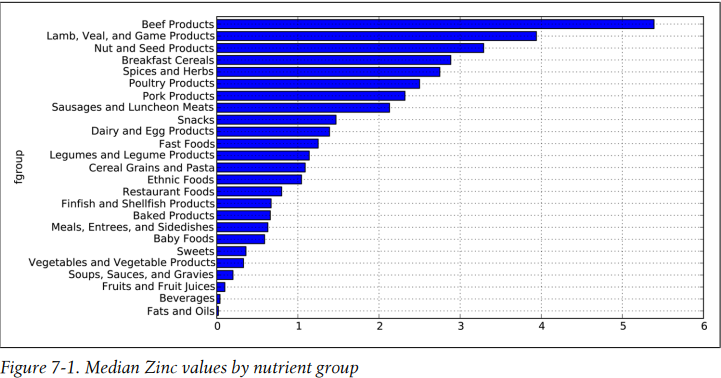
\includegraphics[scale=1.3]{Images/figure.png}
\par\textup{Hiển thị chất dinh dưỡng Animo Acid's ở DataFrame}
\par\quad\textup{In[284]: max\_foods.ix['Amino Acids']['food']}
\par\quad\textup{Out[284]:}
\par\quad\begin{tabular}{ll}
nutrient\\
Alanine &Gelatins, dry powder, unsweetened\\
Arginine& Seeds, sesame flour, low-fat\\
Aspartic& acid Soy protein isolate\\
Cystine& Seeds, cottonseed flour, low fat (glandless)\\
Glutamic acid& Soy protein isolate\\
Glycine& Gelatins, dry powder, unsweetened\\
Histidine& Whale, beluga, meat, dried (Alaska Native)\\
Hydroxyproline& KENTUCKY FRIED CHICKEN, Fried Chicken, ORIGINAL R\\
Isoleucine& Soy protein isolate, PROTEIN TECHNOLOGIES INTERNA\\
Leucine& Soy protein isolate, PROTEIN TECHNOLOGIES INTERNA\\
Lysine& Seal, bearded (Oogruk), meat, dried (Alaska Nativ\\
Methionine& Fish, cod, Atlantic, dried and salted\\
Phenylalanine& Soy protein isolate, PROTEIN TECHNOLOGIES INTERNA\\
Proline& Gelatins, dry powder, unsweetened\\
Serine &Soy protein isolate, PROTEIN TECHNOLOGIES INTERNA\\
Threonine& Soy protein isolate, PROTEIN TECHNOLOGIES INTERNA\\
Tryptophan& Sea lion, Steller, meat with fat (Alaska Native)\\
Tyrosine &Soy protein isolate, PROTEIN TECHNOLOGIES INTERNA\\
Valine& Soy protein isolate, PROTEIN TECHNOLOGIES INTERNA\\
Name: food

\par\end{tabular}

%-	Danh mục TL tham khảo
%-	Phụ lục (nếu có)

\bibliographystyle{plain} % ieeetr
\nocite{*}
\bibliography{refs} 

\end{document}
